\chapter{Release 1: Automatisation des tests de sécurité et amélioration des fonctionnalités de base}
\renewcommand{\thesection}{\arabic{section}}
\begin{justify}
    \vspace{-1.2cm}
    \section*{\texorpdfstring{Introduction}{Introduction}}
    \addcontentsline{toc}{chapter}{\textbf{Introduction}}
    Dans le chapitre précédent, nous avons analysé les besoins et défini le découpage du projet. Cette première release, organisée en deux sprints sur 50 jours, marque le lancement de notre travail selon la méthodologie Scrum. Pour chaque sprint, nous décrivons la phase d’analyse, de conception et de
réalisation.
    \section{Planification de la release 1}
    La release 1 a permis de livrer une première version fonctionnelle de l’application et de préparer l’intégration des modules prévus dans la prochaine version, à travers deux sprints principaux :
\begin{itemize}[label=$\bullet$]
    \item \textbf{Sprint 1.1 : Initialisation, authentification et gestion des permissions (26 jours ouvrés)} : du 3 février 2025 au 11 mars 2025.
    \item \textbf{Sprint 1.2 : Tests de sécurité et notifications (24 jours ouvrés)} : du 12 mars 2025 au 15 avril 2025.
\end{itemize}


    \section{Sprint 1.1 : Initialisation, authentification et gestion des permissions}
Ce premier sprint a couvert quatre axes majeurs :
\begin{itemize}[label=$-$]
    \item \textbf{Initialisation du projet} : création du dépôt Git, configuration des outils de travail, structuration du projet, ainsi que compréhension et analyse du code de l’ancienne application.
    \item \textbf{Développement de la page d’accueil} destinée aux visiteurs.
    \item \textbf{Authentification et gestion des profils} :
    \item \textbf{Gestion des utilisateurs} : développement des fonctionnalités permettant d’afficher la liste des utilisateurs, de consulter leurs informations et de gérer leurs rôles ou autorisations.
\end{itemize}
\subsection{Backlog du sprint 1.1}  
Cette section présente le backlog du sprint 1.1, comme illustré dans le tableau \ref{tab:backlogS11}.
\begin{landscape}
    \renewcommand{\arraystretch}{1.37}
    \begin{spacing}{0.94}
        \begin{longtable}{|p{0.7cm}|p{2.4cm}|p{6cm}|p{1cm}|p{7.2cm}|p{0.2cm}|p{0.2cm}|p{2cm}|}
            \caption{Backlog du sprint 1.1} \label{tab:backlogS11} \\\hline
            \rowcolor{gray!20}
            \textbf{\small ID US} & 
            \multicolumn{1}{c|}{\textbf{\small User Story}} & 
            \multicolumn{1}{c|}{\textbf{\small Description}} & 
            \textbf{\small ID tâche}& 
            \multicolumn{1}{c|}{\textbf{\small Tâches}} & 
            \multicolumn{1}{c|}{\textbf{\small Priorité}} & 
            \multicolumn{1}{c|}{\textbf{\small Risques}} & 
            \textbf{\small Estimation (Jours)}\\\hline
            % ----------- INITIALISATION ------------------
            \hline  
            \rowcolor{blue!20}
			\multicolumn{8}{|c|}{\textbf{EPIC 1: Initialisation du projet}} \\\hline
            1.1 & Installation de l’environnement de travail 
                  & En tant que développeur, je dois installer les outils nécessaires pour travailler. & 1.1.A \newline\vspace{0.5cm} 1.1.B
            & - Installer Python, VSCode, Docker, Git, npm, Angular...\newline
            - Configurer l'environnement. & Élevée & Basse & 1 \\\hline
            1.2 & Formation Scrum. 
                  & En tant que développeur, je dois être formé à la méthodologie Scrum afin d’organiser le travail. 
              & 1.2.A & 
                - Participer à une session de formation SFC de SCRUMstudy. et passer un test pour obtenir la certification.\footnote{Voir annexe B: Figures \ref{fig:ProgressionCours} et \ref{fig:CertifSRC}}
        & Basse & Basse & 2 \\
            \hline
        1.3 & Formation aux tests de pénétration. 
            & En tant que développeur, je dois être formé aux principes du pentesting pour comprendre les besoins de sécurité. 
            & 1.3.A \newline1.3.B 
            & 
            - Étudier les techniques de pentesting. \newline
            - Trouver les principaux outils de base de pentesting Web et les vulnérabilités les plus courantes.
            & Élevée & Basse & 3  \\
            \hline
            1.4 & Formation Selenium. 
                  & En tant que développeur, je dois être formé à l’automatisation avec Selenium pour automatiser les tests fonctionnels. 
                & 1.4.A \newline1.4.B \newline 1.4.C 
                & 
                - Suivre une formation Selenium. \newline
                - Installer et configurer Selenium. \newline
                - Comprendre les bases de la manipulation des éléments Web. 
                & Élevée & Basse & 3 \\\hline
            1.5 & Analyse de la solution existante. 
                  & En tant que développeur, je dois analyser la solution existante pour identifier les fonctionnalités et les limites.
                  & 1.5.A \newline\vspace{0.5cm} 1.5.B 
                & 
                - Analyser la solution existante et identifier ses limites.
                \newline
                - Formaliser les besoins utilisateurs en spécifications fonctionnelles.& Élevée & Moyenne & 3\\
            \hline
            1.6 & Formation RabbitMQ. 
                & En tant que développeur, je dois suivre une formation sur RabbitMQ afin de comprendre le fonctionnement de la communication asynchrone entre services. 
                & 1.6.A \newline\vspace{0.9cm} 1.6.B 
                & 
                - Étudier les concepts de base de RabbitMQ (file d’attente, échange, routage). \newline
                - Installer RabbitMQ en local et tester la communication entre deux services via des files de messages.
                & Élevée & Moyenne & 3 \\
            \hline
            % ----------- CONSULTATION PAGE D’ACCUEIL ------------------
            \hline  
            \rowcolor{blue!20}
            \multicolumn{8}{|c|}{\textbf{EPIC 2: Consultation de la page d’accueil}} \\\hline
            2.1 & Accéder à la page d’accueil 
            & En tant que visiteur, je souhaite accéder à la page d’accueil sans avoir besoin de créer un compte. 
            & 2.1.A 
            &
            - Configurer l’accès libre à la page d’accueil depuis l’URL principale. 
            & Moyenne & Basse & 1/2 \\ \hline
            
            2.2 & Parcourir les sections de la page d’accueil 
            & En tant que visiteur, je souhaite consulter les sections publiques (FAQ, guide utilisateur, services, équipe, tarification, etc.) pour m’informer. 
            & 2.2.A \newline\vspace{0.5cm}2.2.B 
            &
            - Développer les sections publiques avec leur contenu respectif. \newline
            - Intégrer les textes descriptifs, images et icônes explicatives. 
            & Moyenne & Moyenne & 4 \\ \hline
            
            2.3 & Soumettre une demande de contact
            & En tant que visiteur, je souhaite envoyer un message via un formulaire pour poser une question ou obtenir de l’aide. 
            & 2.3.A 
            &
            - Implémenter un formulaire de contact avec champs (nom, e-mail, message) et envoi vers l’administrateur. 
            & Moyenne & Moyenne & 1/2 \\ \hline
            
            % ----------- AUTHENTIFICATION ------------------
            \hline  
            \rowcolor{blue!20}
			\multicolumn{8}{|c|}{\textbf{EPIC 3: Authentification et gestion du profil }} \\\hline
            3.1 & S'inscrire 
            & En tant que visiteur, je dois créer un compte afin d'accéder à l'application. 
            & 3.1.A
            &
            - Implémenter un formulaire d'inscription avec validation et gestion des tokens pour sécuriser les accès. 
            & Moyenne & Moyenne & 1 \\ \hline
            3.2 & Vérifier l’adresse e-mail après l’inscription. 
                & En tant que visiteur, je dois recevoir un lien de vérification afin de valider mon compte et sécuriser l'accès. 
                & 3.2.A \newline\vspace{0.5cm} 3.2.B 
                &
                - Générer un lien de vérification unique après l'inscription. \newline
                - Implémenter un service pour envoyer l'email de vérification. 
                & Moyenne & Moyenne & 1/2 \\ \hline
            3.3 & S’authentifier
                & En tant qu’un utilisateur, je veux pouvoir me connecter pour gérer mon accès. 
                & 3.3.A&
                - Mettre en place une page de connexion avec un formulaire d’authentification et validation des identifiants.
                & Moyenne & Basse & 1/2 \\ \hline
            3.4 & Réinitialiser le mot de passe en cas d’oubli. 
                & En tant qu’un utilisateur, je veux réinitialiser mon mot de passe si je l'oublie, pour retrouver l'accès. 
                & 3.4.A \newline\vspace{0.5cm} 3.4.B 
                &
                - Créer une page de réinitialisation de mot de passe. \newline
                - Implémenter la validation par email pour réinitialiser le mot de passe. 
                & Moyenne & Moyenne & 1 \\ \hline
            3.5 & Gérer le profil utilisateur. 
                & En tant qu’un utilisateur, je veux modifier mes informations personnelles pour garder mes données à jour. 
                & 3.5.A \newline\vspace{0.5cm} 3.5.B 
                &
                - Créer une page pour modifier les informations personnelles. \newline
                - Implémenter la mise à jour des utilisateur dans la base de données. 
                & Moyenne & Moyenne & 1/2 \\\hline
              3.6 & Se déconnecter 
                & En tant qu’un utilisateur, je veux me déconnecter de l’application.
                & 3.6.A
                &
                - Implémenter un bouton de déconnexion sur l’interface frontend avec suppression du jeton de session. 
                & Moyenne & Basse & 1/2 \\  \hline
            \hline     
            % ---- GESTION DES UTILISATEURS -----------
            \hline  
            \rowcolor{blue!20}
			\multicolumn{8}{|c|}{\textbf{EPIC 11: Gestion des utilisateurs}} \\\hline
            11.1 & Rechercher un utilisateur 
            & En tant qu’administrateur, je souhaite rechercher un utilisateur avec différents filtres pour retrouver rapidement un profil. 
            & 11.1.A 
            & - Implémenter un champ de recherche avec filtres (nom, email, rôle…). 
            & Élevée & Moyenne & 1/2 \\\hline
            
            11.2 & Exporter la liste des utilisateurs 
            & En tant qu’administrateur, je souhaite exporter la liste des utilisateurs afin de la conserver.
            & 11.2.A 
            & - Générer un export (PDF/CSV/HTML /JSON) de la liste des utilisateurs. 
            & Moyenne & Basse & 1/2 \\\hline
            
            11.3 & Consulter la liste des utilisateurs 
            & En tant qu’administrateur, je souhaite voir la liste des utilisateurs pour une vue globale. 
            & 11.3.A 
            & - Afficher un tableau paginé listant les comptes avec leurs informations principales. 
            & Moyenne & Basse & 1/4 \\\hline
            11.4 & Supprimer un utilisateur 
            & En tant qu’administrateur, je souhaite pouvoir supprimer un utilisateur du système. 
            & 11.4.A 
            & - Ajouter un bouton de suppression avec confirmation de sécurité. 
            & Élevée & Moyenne & 1/4 \\\hline
            
            11.5 & Gérer les permissions des utilisateurs
            & En tant qu’administrateur, je souhaite attribuer, modifier ou révoquer les permissions d’un utilisateur afin de contrôler ses droits d’accès.
            & 11.5.A 
            \newline\vspace{1.9cm} 11.5.B
             \newline\vspace{0.5cm} 11.5.C
            & - Créer une interface permettant d’attribuer, modifier, révoquer et visualiser les permissions d’accès aux différents types de scans (fonctionnel, SEO, sécurité) pour chaque utilisateur.\newline
            - Implémenter des vérifications côté backend sur les routes sensibles.\newline
            - Restreindre l’accès selon les permissions via des guards côté frontend.
            & Élevée & Moyenne & 1/2 \\\hline

            \rowcolor{gray!20}
			\multicolumn{7}{|c|}{TOTAL} &  26UE \\
            \hline 
        \end{longtable}
    \end{spacing}
    \vspace{-0.1cm}
\end{landscape}

\subsection{Analyse du sprint 1.1}
Nous passons à la phase d’analyse de ce sprint afin de présenter le diagramme de cas d’utilisation de ce sprint ainsi que les descriptions textuelles de quelques cas d’utilisation. 
\subsubsection{Diagramme de cas d’utilisation du sprint 1.1}
La figure \ref{fig:caseS1} présente le diagramme de cas d’utilisation raffiné du sprint 1.1, mettant en évidence les cas d’usage correspondant aux fonctionnalités attendues à la fin de ce sprint.
\begin{figure}[H]
    \centering
    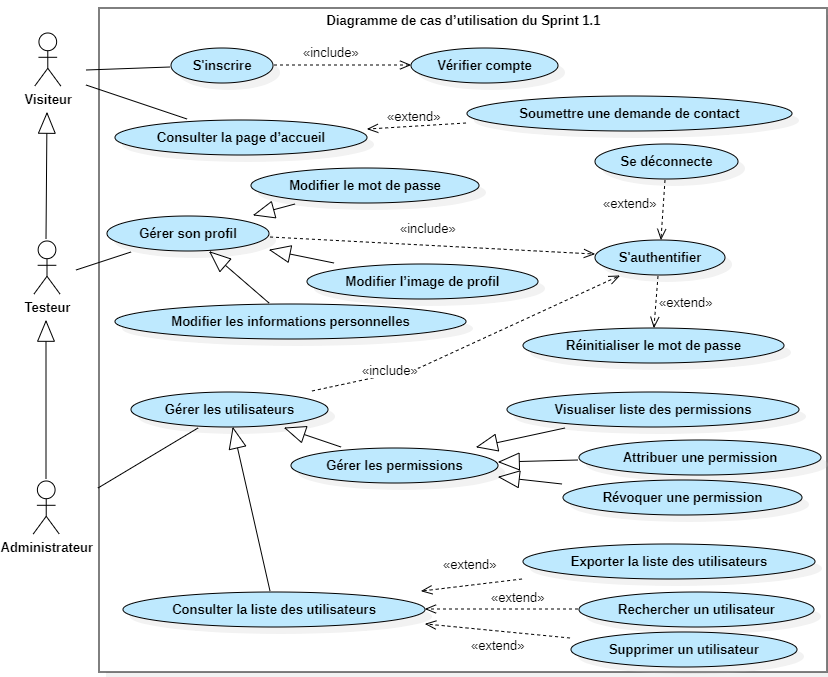
\includegraphics[width=0.92\linewidth]{chapitres/ch3Sp1/section/sprint1/img/LastUseCaseSprint1.1.png}
    \caption{Diagramme de cas d’utilisation du sprint 1.1}
    \label{fig:caseS1}
\end{figure}
\vspace{-0.5cm}
\subsubsection{Raffinement des cas d’utilisation}
Cette étape a permis de mieux comprendre les interactions, de repérer les dépendances et de découper les fonctionnalités.
\begin{enumerate}[label=\alph*), left=-0.1cm]
    \item \textbf{Raffinement du cas d’utilisation «S'inscrire»:}\\
        L'inscription inclut la saisie et validation des informations, la confirmation par e-mail avec un code OTP et la gestion des erreurs pour garantir une expérience utilisateur optimale.
        \begin{itemize}[label=\ding{111}, left=-0.1cm]
            \item \textbf{Description textuelle du cas d’utilisation "S'inscrire":} \\
                  Le tableau ~\ref{tab:descInsc}  présente la description textuelle du cas d’utilisation "S'inscrire".
                  \begin{spacing}{1.1}
                        \begin{longtable}{|p{0.12\linewidth}|p{0.88\linewidth}|}
                            \caption{Description textuelle du cas d’utilisation : S'inscrire}
                            \label{tab:descInsc}\\
                            \hline
                            \textbf{Titre} & S'inscrire \\
                            \hline
                            \textbf{Acteur} & Visiteur \\
                            \hline
                            \textbf{Résumé} & Ce cas d'utilisation décrit le processus d'inscription permettant au visiteur de créer un compte personnel. \\
                            \hline
                            \textbf{Pré-conditions} & 
                                Le visiteur doit disposer d’un accès à Internet via un dispositif connecté (ordinateur, tablette, smartphone). \\
                            \hline
                            \textbf{Post-conditions} & 
                                Un nouveau compte utilisateur est créé, et un email de confirmation contenant un code OTP est envoyé afin de vérifier l’adresse email saisie. \\
                            \hline
                            \textbf{Scénario nominal} & 
                            \begin{minipage}{\linewidth}
                                \vspace{0.1cm}
                                \begin{enumerate}[label=\arabic*., left=-0.05cm]
                                    \item Le visiteur accède à la page d'inscription et clique sur le bouton "Inscrire".
                                    \item Le système affiche un formulaire de saisie des informations d'inscription.
                                    \item Le visiteur remplit le formulaire avec ses informations, puis le soumet.
                                    \item Le système valide les informations fournies.
                                    \item Le système enregistre les données du visiteur dans la base de données.
                                    \item Il génère automatiquement des identifiants de connexion.
                                    \item Le système envoie un e-mail de confirmation contenant un code OTP (One-Time Password) de 6 chiffres.
                                    \item L'utilisateur saisit ce code dans un champ dédié.
                                    \item Une fois le code validé avec succès, l'adresse e-mail est vérifiée et l'inscription est finalisée.
                                \end{enumerate}
                                \vspace{0.05cm}
                            \end{minipage}\\
                            \hline
                            \textbf{Scénario d’erreur} &
                            \begin{minipage}{\linewidth}
                                \vspace{0.1cm}
                                \begin{itemize}[left=0cm]
                                    \item[\textbullet] \textbf{Étape 4 (Informations incomplètes):}
                                    \begin{itemize}[label=\ding{56}]
                                        \item Si des champs obligatoires sont laissés vides, le système affiche un message d’erreur précisant les champs à compléter.
                                        \item L'utilisateur est invité à fournir les informations manquantes.
                                    \end{itemize}
                        
                                    \item[\textbullet] \textbf{Étape 4 (Annulation) :}
                                    \begin{itemize}[label=\ding{56}]
                                        \item L'utilisateur peut annuler l'inscription avant la soumission. Aucun enregistrement n’est effectué.
                                    \end{itemize}
                        
                                    \item[\textbullet] \textbf{Étape 7 (Erreur d'enregistrement):}
                                    \begin{itemize}[label=\ding{56}]
                                        \item En cas d’échec lors de l’enregistrement des données, le système affiche un message d’erreur et invite à réessayer ultérieurement.
                                    \end{itemize}
                        
                                    \item[\textbullet] \textbf{Étape 9  (Expiration du code OTP) :}
                                    \begin{itemize}[label=\ding{56}]
                                        \item Le code OTP possède une durée de validité limitée. En cas de dépassement, un message informe l’utilisateur de l’expiration du code et lui propose d’en générer un nouveau via le lien contenu dans l’e-mail.
                                    \end{itemize}
                        
                                    \item[\textbullet] \textbf{Étape 10 (Code OTP incorrect):}
                                    \begin{itemize}[label=\ding{56}]
                                        \item Si l'utilisateur saisit un code OTP erroné, le système affiche un message d'erreur et l'invite à le ressaisir.
                                        \item Après plusieurs tentatives échouées, le système bloque temporairement la validation par OTP et propose l'envoi d'un nouveau code.
                                    \end{itemize}
                                \end{itemize}
                                \vspace{0.1cm}
                            \end{minipage}\\
                            \hline
                        \end{longtable}
                    \end{spacing}
                  \vspace{-0.2cm}
            \item \textbf{Diagramme  de séquence du cas d’utilisation "S'inscrire":} \\ Les étapes de déroulement du cas d’utilisation "S'inscrire" sont décrites par le diagramme de séquence illustré par la figure ~\ref{fig:seqInscrire}.
            \begin{figure}[H]
                \centering
                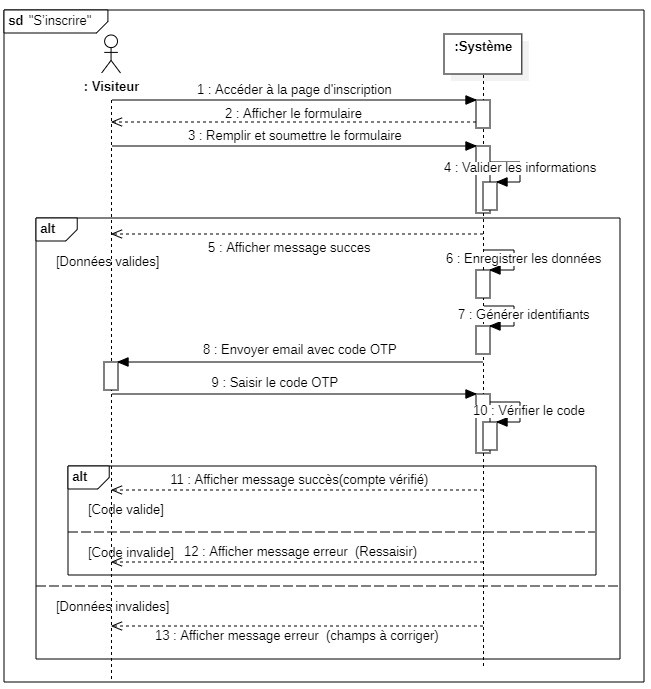
\includegraphics[width=0.9\textwidth]{chapitres/ch3Sp1/section/sprint1/img/seq-creer-compte-sp1.png}
                \caption{Diagramme de séquence du cas d’utilisation de "S'inscrire"}
                \label{fig:seqInscrire}
            \end{figure}
        \end{itemize}
    
  \item \textbf{Raffinement du cas d’utilisation « Gérer les permissions des utilisateurs » :}\\
    Cette section détaille le raffinement du cas d’utilisation « Gérer les permissions des utilisateurs ». Ce cas d’utilisation permet à un administrateur de gérer les droits d’accès des utilisateurs aux différentes permissions (fonctionnel, SEO, sécurité...).
     \begin{itemize}[label=\ding{111}, left=-0.1cm]
            \item \textbf{Description textuelle du cas d’utilisation "Attribuer des permissions" :}\\
            Le tableau \ref{tab:descAttribuerPermissions} décrit textuellement le cas d’utilisation <<Attribuer des permissions>>.
            \begin{spacing}{1.2}
                \begin{longtable}{|p{0.12\linewidth}|p{0.88\linewidth}|}
                \caption{Description textuelle du cas d’utilisation : Attribuer des permissions}
                \label{tab:descAttribuerPermissions} \\
                \hline
                \textbf{Titre} & Attribuer des permissions \\
                \hline
                \textbf{Acteur} & Administrateur \\
                \hline
                \textbf{Résumé} & Ce cas d'utilisation permet à l’administrateur d’attribuer à un utilisateur des permissions d’accès aux tests (fonctionnel, SEO, sécurité). \\
                \hline
                \textbf{Pré-conditions} & L’utilisateur concerné doit exister dans le système. L’administrateur doit être connecté. \\
                \hline
                \textbf{Post-conditions} & Les permissions sélectionnées sont enregistrées et appliquées à l’utilisateur dans la base de données. \\
                \hline
                \textbf{Scénario nominal} &
                \begin{minipage}{\linewidth}
                \vspace{0.1cm}
                \begin{enumerate}[label=\arabic*., left=0.2cm]
                    \item L’administrateur accède à l’interface de gestion des permissions.
                    \item Il sélectionne un utilisateur.
                    \item Il choisit les permissions à autoriser.
                    \item Il valide la configuration.
                    \item Le système enregistre les nouvelles permissions.
                \end{enumerate}
                \vspace{0.1cm}
                \end{minipage} \\
                \hline
                \textbf{Scénario d’erreur} &
                \begin{minipage}{\linewidth}
                    \vspace{0.1cm}
                    \begin{itemize}[left=0cm]
                        \item[\textbullet] \textbf{Erreur d’enregistrement :} En cas d’échec d’écriture en base de données, le système signale une erreur et annule l’opération.
                    \end{itemize}
                    \vspace{0.1cm}
                \end{minipage} \\
                \hline
                \end{longtable}
            \end{spacing}
            \vspace{-0.2cm}
            \item  \textbf{Diagramme d’activité : Vérification des permissions d’accès:}\\
                Le diagramme d’activité de la figure \ref{fig:permission-activite} illustre le processus de gestion conditionnelle des droits d’accès. Après l’authentification, le système accorde aux administrateurs un accès complet leur permettant d’attribuer des permissions.
            \begin{figure}[H]
        \centering
        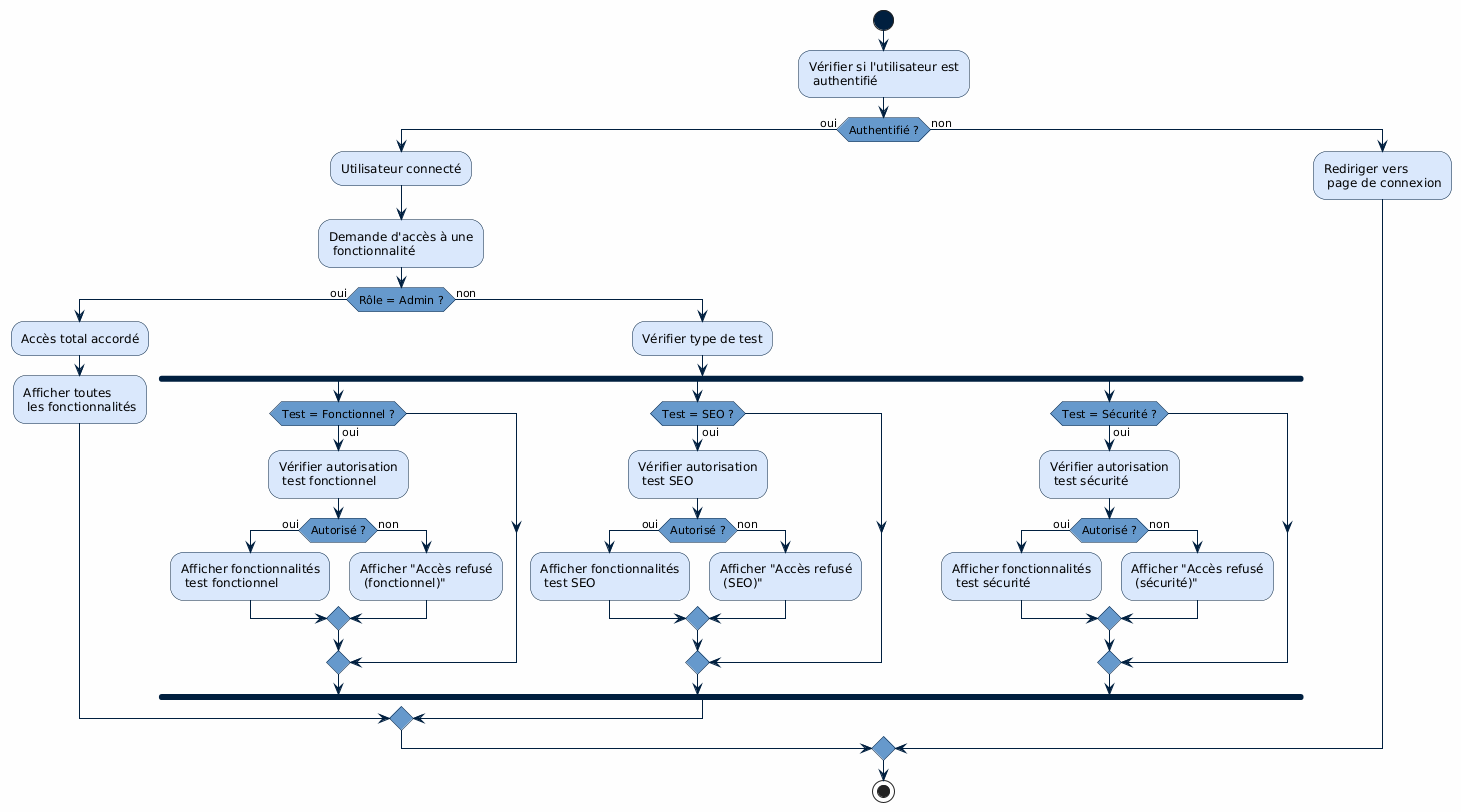
\includegraphics[width=\linewidth]{chapitres/ch3Sp1/section/sprint1/img/permission-activite.png}
        \caption{\centering Diagramme d’activité : Processus de vérification des permissions lors de la demande d’accès à une fonctionnalité}
        \label{fig:permission-activite}
    \end{figure}
    \end{itemize}
    \vspace{-0.5cm}
\end{enumerate}

\subsection{Conception du sprint 1.1}
La conception de ce sprint commence par la présentation du diagramme de classes, représentant la structure du système.
\subsubsection{Diagramme de classe du sprint 1.1}
La figure \ref{fig:classsp1} illustre le diagramme de classes du sprint 1.1, représentant les principales entités métier, leurs attributs, leurs méthodes, ainsi que les relations entre elles.
\begin{figure}[H]
    \centering
    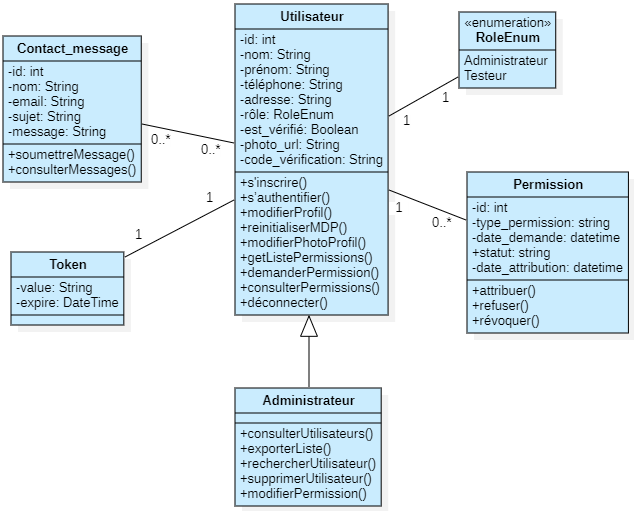
\includegraphics[width=0.9\linewidth]{chapitres/ch3Sp1/section/sprint1/img/classeL1-SP1.1.png}
    \caption{Diagramme de classe du sprint 1.1}
    \label{fig:classsp1}
\end{figure}
\vspace{-0.4cm}
Les principales classes modélisées de sprint 1.1 sont les suivantes:
    \begin{itemize}[label=$*$]
       \item \textbf{Utilisateur :} Représente les comptes utilisateurs de l’application. Elle contient des informations personnelles (nom, prénom, téléphone, adresse, email, mot de passe, et rôle (\texttt{RoleEnum}) ainsi que des méthodes relatives à la gestion du compte et d’administration des utilisateurs.
       \item \textbf{Contact\_message :} Permet aux utilisateurs de soumettre des messages via un formulaire de contact. Elle comprend des attributs et des méthodes pour stocker les détails du message.
       \item \textbf{RoleEnum (énumération) :} Définit les différents rôles possibles dans l’application, notamment \textit{Administrateur} et \textit{Testeur}, utilisés pour la gestion des droits d’accès.
       \item \textbf{Permission :} Représente les permissions associées aux utilisateurs, avec les attributs suivants : type de permission, date de demande, date d’attribution, statut, ainsi que les méthodes : révoquer, attribuer et refuser une demande de permission.
       \item \textbf{Token :} Modélise un jeton d’authentification, avec ses valeurs et sa date d’expiration, utilisé pour la gestion des sessions utilisateurs.
       \item \textbf{Administrateur :} Hérite de la classe Utilisateur et dispose de méthodes spécifiques pour la gestion des utilisateurs, comme consulter la liste des utilisateurs, rechercher, modifier leurs permissions, supprimer des utilisateurs, et exporter la liste.
    \end{itemize}
Les associations entre classes sont également représentées dans le diagramme, notamment:
\begin{itemize}[label=$-$, left=0.05cm]
    \item Un \texttt{Utilisateur} possède un rôle défini par \texttt{RoleEnum} et peut avoir plusieurs \texttt{Permission}.
    \item Un \texttt{Administrateur} : utilisateur disposant de privilèges étendus pour la gestion des autres comptes.
    \item Un \texttt{Utilisateur} peut générer un ou plusieurs \texttt{Token} pour gérer ses sessions.
    \item Un \texttt{Utilisateur} peut envoyer un \texttt{Contact\_message} à plusieurs administrateurs, tandis qu’un \texttt{Administrateur} peut recevoir des messages envoyés par plusieurs utilisateurs.
\end{itemize}
Ce diagramme constitue une base essentielle pour la suite du développement, en assurant une structure cohérente et maintenable du code tout au long des itérations agiles.


\subsection{Réalisation du sprint 1.1}
Dans cette section, nous présentons les principales interfaces développées durant ce premier sprint, en commençant par la page d’accueil, puis celles liées au module d’authentification, et enfin les interfaces de contact et d'administration des utilisateurs.
\begin{itemize}[label=$\bullet$]
    \item  \textbf{Interface de la page d’accueil}: Les figures\footnote{Voir annexe E : Figures \ref{fig:accueil} et \ref{fig:accueil2}} \ref{fig:accueil} et \ref{fig:accueil2} illustrent l’interface de la page d’accueil de l’application. Celle-ci offre un aperçu général du système, avec un design moderne et une navigation intuitive, permettant aux utilisateurs de découvrir rapidement les principales fonctionnalités de la plateforme.
    \item \textbf{Interface d’inscription}:
        La figure~\ref{fig:register} illustre l’interface d’inscription. Elle permet à un nouvel utilisateur de créer un compte en renseignant ses informations personnelles. Des contrôles de saisie assurent la validation des données entrées.  
        \begin{figure}[H]
            \centering
            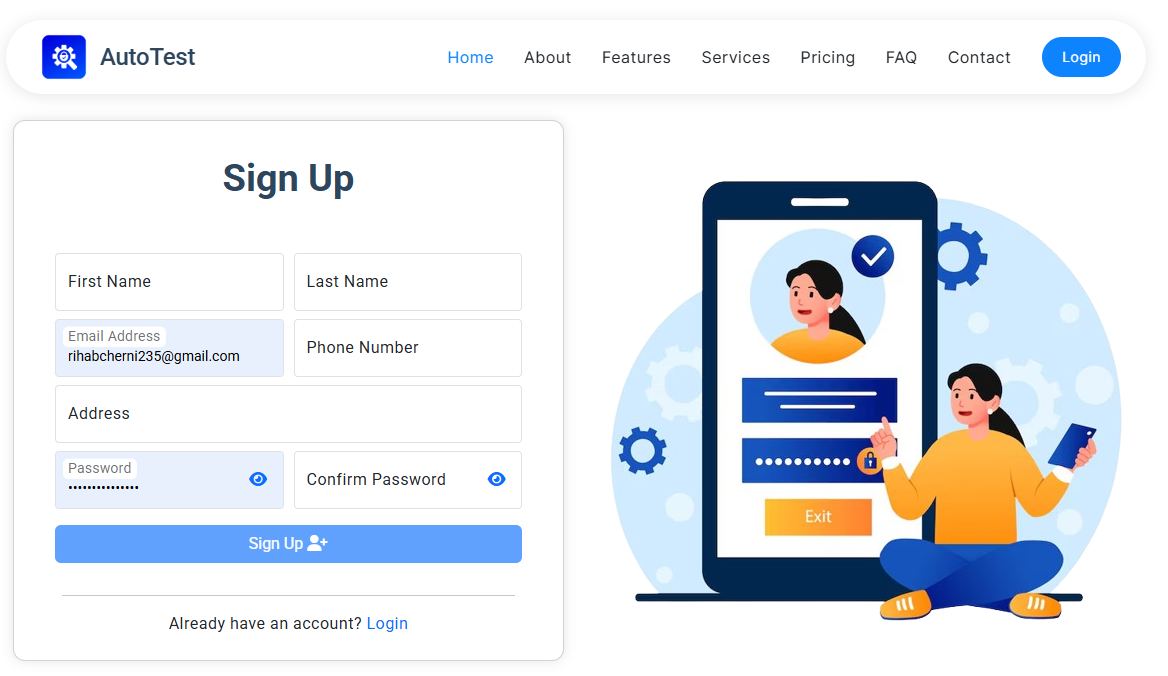
\includegraphics[width=\linewidth]{chapitres/ch3Sp1/section/sprint1/img/interface/register.png}
            \caption{\centering Interface d'inscription}
            \label{fig:register}
        \end{figure}
        \vspace{-0.3cm}
    \item \textbf{Interface de connexion}:
        La figure~\ref{fig:login}\footnote{Voir annexe E: Figures \ref{fig:login}} présente l’interface de connexion. Elle permet à l’utilisateur de s’authentifier via son e-mail et son mot de passe. Des vérifications sont mises en place pour gérer les erreurs (identifiants invalides, champs manquants...).
    \item \textbf{Vérification par e-mail (OTP)}:
        Après l’inscription, l’utilisateur reçoit un e-mail contenant un code de vérification. Les figures \ref{fig:email-verif}\footnote{Voir annexe E: Figures \ref{fig:email-verif}} et \ref{fig:email-verification}\footnote{Voir annexe E: Figures \ref{fig:email-verification}} présentent l’interface de réception et de saisie du code.
    \item \textbf{Mot de passe oublié et réinitialisation}:
        Le système inclut une fonctionnalité de récupération de mot de passe. Les interfaces correspondantes sont illustrées dans les figures~\ref{fig:forgot-password}\footnote{Voir annexe E: Figures \ref{fig:forgot-password}},~\ref{fig:reset-password-email}\footnote{Voir annexe E: Figures \ref{fig:reset-password-email}} et~\ref{fig:reset-password}\footnote{Voir annexe E: Figures \ref{fig:reset-password}}.
        \item \textbf{Profil utilisateur} : La figure~\ref{fig:profile} présente l’interface du profil utilisateur. Chaque utilisateur peut consulter et modifier ses informations personnelles (nom, image de profil, etc.), ainsi que visualiser les permissions qui lui sont attribuées. \\ Un bouton dédié permet également à l’utilisateur de soumettre une demande d’accès à des permissions supplémentaires via une boîte de dialogue affichant la liste des permissions disponibles, que l’utilisateur peut sélectionner avant de valider sa demande.
         \begin{figure}[H]
                \centering
                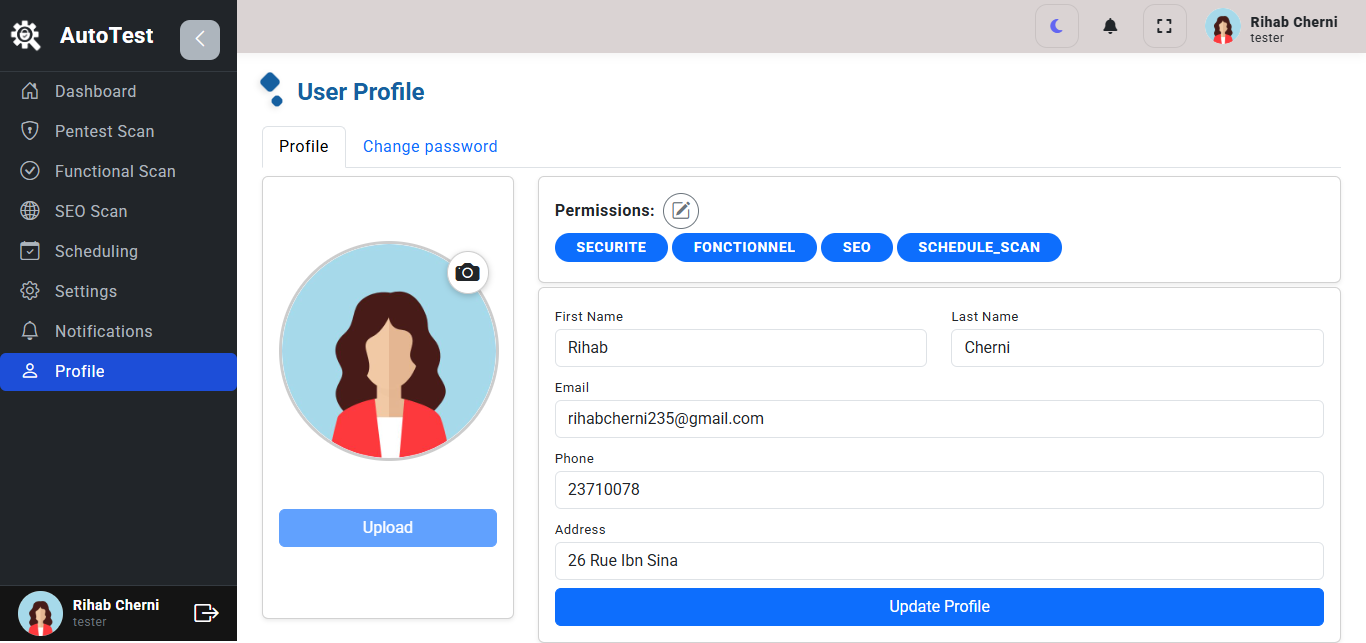
\includegraphics[width=\linewidth]{chapitres/ch3Sp1/section/sprint1/img/interface/profile.png}
                \caption{\centering Interface du profil utilisateur}
                \label{fig:profile}
            \end{figure}
        \vspace{-0.3cm}
    \item \textbf{Gestion des utilisateurs et permissions}:
        La figure~\ref{fig:gestionUser} présente l’interface dédiée à la gestion des utilisateurs pour l’administrateur. Elle permet de visualiser, rechercher, modifier ou supprimer les comptes utilisateurs, de gérer les permissions attribuées à chacun, et d’exporter la liste aux différents formats disponibles.
        \begin{figure}[H]
            \centering
            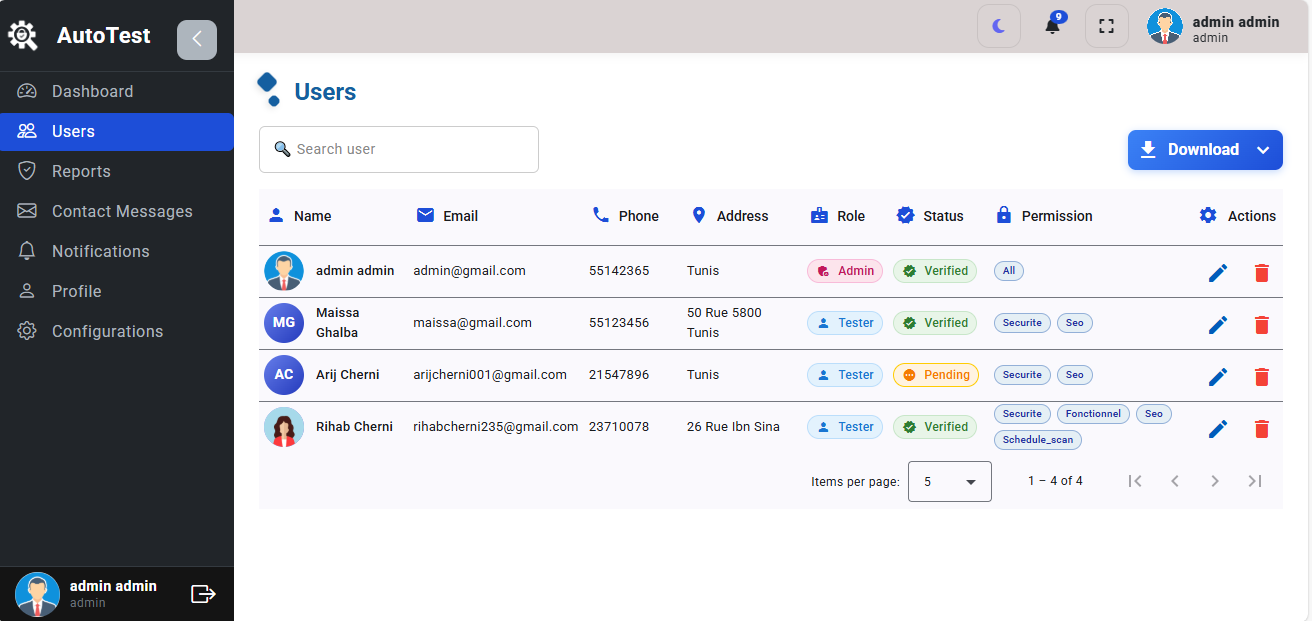
\includegraphics[width=\linewidth]{chapitres/ch3Sp1/section/sprint1/img/interface/user-liste.PNG}
            \caption{\centering Interface de gestion des utilisateurs et permissions (admin)}
            \label{fig:gestionUser}
        \end{figure}
        \vspace{-0.3cm}
       \item \textbf{Interfaces liées à la gestion des permissions et guards} :
Cette partie décrit les interfaces conditionnées par le système de gestion des permissions et les guards de sécurité implémentés dans l’application.
\begin{itemize}[label=$\diamond$, left=0.01cm]
    \item \textbf{Menu latéral dynamique selon les permissions} : La figure~\ref{fig:sidebar}\footnote{Voir annexe E : Figure~\ref{fig:sidebar}} illustre l’adaptation dynamique du menu latéral en fonction des droits d’accès de l’utilisateur. Trois cas sont représentés : (a) un utilisateur sans permissions, où seuls les éléments de base (profil, paramètres) sont visibles, (b) un utilisateur disposant de permissions spécifiques accédant uniquement aux modules autorisés, et (c) un utilisateur avec l’ensemble des droits, ayant un accès complet aux modules (SEO, sécurité, tests fonctionnels, génération de rapports, ...).
        \item \textbf{Interfaces de gestion des permissions}: La figure~\ref{fig:permission-interfaces}\footnote{Voir annexe E: Figures \ref{fig:permission-interfaces}} présente les interfaces illustrant les mécanismes de gestion et de demande de permissions.    
        \begin{itemize}[label=$*$, left=0.01cm]
            \item (a) Boîte de dialogue des permissions pour l’administrateur, avec toutes les permissions cochées et désactivées grâce à la permission spéciale \texttt{tous}, accordant un accès complet.
            \item (b) Boîte de dialogue d’édition des permissions, accessible uniquement à l’administrateur, permettant d’ajouter ou de révoquer dynamiquement les droits d’un utilisateur de rôle \texttt{testeur}.
            \item (c) Interface de demande de permissions, permettant au testeur de visualiser les accès manquants et de soumettre une requête à l’administrateur. Une notification est automatiquement envoyée. Ce composant a été conçu avec une logique évolutive en vue de la commercialisation de l’application : certaines permissions pourront, à l’avenir, être conditionnées par un abonnement payant. Une option de paiement ou un lien vers la facturation pourra alors s’activer dynamiquement lors de la sélection.
    \end{itemize}
\end{itemize}
\item \textbf{Soumettre un message de contact}:
        L’interface illustrée dans la figure~\ref{fig:contact}\footnote{Voir annexe E: Figures \ref{fig:contact}} permet à tout utilisateur (même non connecté) de soumettre un message à l’administrateur.
    \item \textbf{Interface de liste des messages (côté administrateur)}:
        La figure~\ref{fig:admin-contact-list}\footnote{Voir annexe E: Figures \ref{fig:admin-contact-list}} montre l’interface accessible uniquement à l’administrateur, lui permettant de consulter la liste des messages reçus via le formulaire de contact.
\end{itemize}

    \section{Sprint 1.2 : Tests de sécurité et notifications}
Ce sprint a permis d’ajouter des fonctionnalités essentielles en matière de sécurité et d’interaction avec les utilisateurs :
\begin{itemize}[label=$-$]
    \item \textbf{Gestion des scans de tests de sécurité} : développement d’un module permettant d’analyser les vulnérabilités des sites web.
    \item \textbf{Paramétrage des canaux de diffusion des rapports de tests} : mise en place d’un système de configuration des moyens de communication des résultats (email, Slack, Jira).
    \item \textbf{Notifications en temps réel} : ajout d’un système de notifications permettant d’alerter les utilisateurs lors de la fin d’un scan ou lors de la détection d’une anomalie.
\end{itemize}
\subsection{Backlog du sprint 1.2}  
Dans cette section, nous présentons le backlog du sprint 1.2, tel qu'illustré dans le tableau \ref{tab:backlogS22}.
Ce backlog détaille les besoins sélectionnées pour ce sprint, accompagnées de leurs tâches associées, priorités, risques et estimations en jours.
\begin{landscape}
    \renewcommand{\arraystretch}{1.3}
    \begin{spacing}{0.94}
        \begin{longtable}{|p{0.6cm}|p{2.6cm}|p{4.9cm}|p{0.97cm}|p{8.6cm}|p{0.35cm}|p{0.35cm}|p{1.6cm}|}
            \caption{Backlog du sprint 1.2} \label{tab:backlogS22} \\\hline
            \rowcolor{gray!20}
            \textbf{\small ID US} & 
            \multicolumn{1}{c|}{\textbf{\small User Story}} & 
            \multicolumn{1}{c|}{\textbf{\small Description}} & 
            \textbf{\small ID tâche}& 
            \multicolumn{1}{c|}{\textbf{\small Tâches}} & 
            \multicolumn{1}{c|}{\textbf{\small Priorité}} & 
            \multicolumn{1}{c|}{\textbf{\small Risques}} & 
            \textbf{\fontsize{9}{11}\selectfont Estimation (Jours)}\\\hline
            % ----------- SCANS DE SÉCURITÉ ------------------
			\rowcolor{blue!20}
            \multicolumn{8}{|c|}{\textbf{EPIC 4: Gestion des scans de tests de sécurité d’un site web}} \\\hline
            
            4.1 & Configurer les paramètres de scan selon les besoins. & En tant que testeur, je veux personnaliser les paramètres de scan pour adapter les analyses aux besoins spécifiques. 
            & 4.1.A \newline\vspace{0.5cm} 4.1.B &
            - Développer une interface pour configurer les paramètres de scan. \newline
            - Permettre à l’utilisateur de choisir la profondeur des scans. & Moyenne & Moyenne & 1/2\\ \hline

           4.2 & Sélectionner les outils de sécurité à utiliser pour l’analyse.
            & En tant que testeur, je veux choisir les outils à utiliser afin d’adapter l’analyse aux besoins de la cible, enregistrer mes préférences et les réutiliser lors des scans suivants.
             & 4.2.A \newline\vspace{1.9cm} 4.2.B&
            - Développer une interface avec des cases à cocher permettant de sélectionner les outils souhaités avant le lancement d’un scan avec une sélection multiple et des boutons « Tout sélectionner » / « Tout désélectionner ».\newline
            - Enregistrer les outils préférés de chaque utilisateur dans la base de données et les recharger automatiquement pour les scans suivants.
            & Élevée  & Élevée  & 1\\ \hline
            
            4.3 & Lancer un scan de test de sécurité. & En tant que testeur, je veux initier un scan de test de sécurité sur une cible pour identifier ses vulnérabilités. 
            & 
            4.3.A \newline\vspace{1cm} 
            4.3.B\newline\vspace{0.9cm} 
            4.3.C\newline\vspace{0.5cm} 
            4.3.D\newline\vspace{0.5cm} 
            4.3.E\newline\vspace{0.5cm} 
            4.3.F\newline\vspace{0.5cm} 
            4.3.G&
            - Développer une interface de lancement de scan avec champ URL de la cible à tester, les outils, paramètres de scan et bouton "Lancer".\newline
            - Corriger l'automatisation des outils existants \textbf{ZAP} et \textbf{Wapiti} en vérifiant leur configuration et optimisant les paramètres de détection.\newline
            - Intégrer et automatiser l’exécution d’outils spécialisés tels que SQLMap, Nuclei, Nmap...\newline
            - Utiliser le multithreading pour exécuter les outils en parallèle.\newline
            - Unifier les formats de sortie pour générer un rapport commun.\newline
            - Créer une base de données des vulnérabilités détectées.\newline
            - Générer un rapport JSON unifié via un modèle d’agrégation et de comparaison.
            & Élevée & Moyenne & 1 \\ \hline
            
            4.4 & Lancer un scan de sécurité avec authentification dynamique. 
                & En tant que testeur, je souhaite initier un scan authentifié afin d’identifier les vulnérabilités présentes dans les zones protégées.  & 4.4.A \newline\vspace{0.5cm} 4.4.B  & 
                - Intégrer l’authentification dynamique pour chaque outil. \newline
                - Tester les mécanismes d’authentification pour chaque outil (cookies, jetons, mots de passe). & Élevée & Moyenne &3 \\ \hline
            
            4.5 & Planifier des scans  de test sécurité automatiques. 
                & En tant que testeur, je veux définir une planification automatique des scans pour assurer une surveillance régulière. & 4.5.A \newline\vspace{0.5cm} 4.5.B  &
                - Créer une interface de planification pour automatiser les scans. \newline
                - Tester le bon déroulement des scans planifiés. & Élevée & Moyenne & 1 \\ \hline
                
            4.6 & Suivre la progression du scan en temps réel via WebSocket. 
                & En tant que testeur, je veux visualiser en temps réel l’évolution des scans pour suivre leur progression.
                & 4.6.A \newline 4.6.B &
                - Intégrer WebSocket pour suivre la progression. \newline
                - Mettre à jour l'interface utilisateur avec des informations en temps réel.  & Élevée & Moyenne & 1 \\ \hline            
            4.7 & Visualiser les résultats des scans. 
                    & En tant que testeur, je peux consulter les résultats afin d'analyser la sécurité de l'application. 
                    & 4.7.A \newline\vspace{0.5cm} 4.7.B
                    & 
                    - Implémenter une interface pour visualiser les résultats des scans. \newline
                    - Fournir des options de filtrage pour faciliter l'analyse des résultats. 
                    & Élevée & Basse & 2 \\
                \hline
            4.8 & Accéder à l’historique des scans précédents. 
                    & En tant que testeur, je dois accéder aux rapports des anciens scans pour suivre l'évolution des vulnérabilités et conserver une trace des analyses précédentes.
                    & 4.8.A 
                    \newline 4.8.B
                    \newline\vspace{0.5cm} 4.8.C
                    \newline 4.8.D
                    \newline\vspace{0.4cm} 4.8.E
                    \newline\vspace{0.5cm} 4.8.F
                    \newline\vspace{0.cm} 4.8.G
                    & 
                     - Afficher les historiques de scans.\newline
                     - Ajouter une pagination pour naviguer entre les pages de résultats.\newline
                     - Ajouter des filtres (par type, outil, gravité...). \newline
                     - Implémenter une barre de recherche pour retrouver un scan précis.\newline
                     - Ajouter une option de suppression pour chaque rapport.\newline
                     - Permettre l'accès aux détails d’un scan : liste des vulnérabilités par outil et les logs associés à chaque scan.\newline
                     - Afficher un résumé global du scan accompagné de la liste complète des vulnérabilités détectées pour chaque scan.
                    & Moyenne & Basse & 1 \\
                \hline
                4.9 & Télécharger les rapports aux formats JSON, PDF et CSV. 
                    & En tant que testeur, je dois télécharger les rapports sous différents formats pour faciliter leur traitement et archivage. 
                    & 4.9.A \newline\vspace{0.5cm} 4.9.B
                    & 
                    - Développer des options d'exportation pour les rapports. \newline
                    - Ajouter des boutons pour télécharger les rapports en formats JSON, PDF et CSV.
                    & Moyenne & Moyenne & 1 \\
                \hline
                4.10 & Intégrer et visualiser les rapports via Jira. 
                    & En tant que testeur, je dois intégrer les résultats dans Jira pour créer des tickets et assurer un suivi structuré des incidents détectés. 
                    & 4.10.A \newline\vspace{0.5cm} 4.10.B
                    & 
                    - Créer une intégration avec Jira pour la création automatique de tickets. \newline
                    - Visualiser les résultats dans des dashboards Jira.
                    & Élevée & Élevée & 3/2 \\
                \hline
                4.11 & Accéder aux rapports via Slack. 
                    & En tant que testeur, je dois recevoir les rapports via Slack pour une communication rapide au sein de l'équipe. 
                    & 4.11.A \newline\vspace{0.5cm} 4.11.B
                    & 
                    - Mettre en place une intégration avec Slack pour envoyer les rapports. \newline
                    - Ajouter des notifications Slack pour chaque scan terminé.
                    & Moyenne & Basse & 3/2 \\
                \hline
                4.12 & Recevoir les rapports directement par e-mail. 
                    & En tant que testeur, je dois recevoir automatiquement les rapports par e-mail pour assurer leur disponibilité hors plateforme. 
                    & 4.12.A \newline\vspace{0.5cm}4.12.B
                    & 
                    - Configurer l'envoi automatique de rapports par e-mail. \newline
                    - Ajouter un modèle d'e-mail pour l'envoi des rapports.
                    & Moyenne & Basse & 3/2 \\
                \hline
                4.13 & Détecter automatiquement les pages de login, en excluant les pages d’inscription. 
                    & En tant que testeur, je souhaite que le système identifie automatiquement les pages d’authentification d’un site pour configurer correctement les scans authentifiés. 
                    & 4.13.A \newline\vspace{0.5cm} 4.13.B
                    & 
                    - Analyser le code HTML des pages pour détecter les formulaires de connexion.\newline
                    - Mettre en place des règles pour exclure les pages d’inscription et les pages non pertinentes.
                    & Élevée & Moyenne & 2 \\
                \hline
                4.14 & Annuler un scan de sécurité en cours. 
                    & En tant que testeur, je souhaite pouvoir annuler un scan de sécurité en cours d'exécution afin d’arrêter une analyse inutile ou incorrectement configurée.
                    & 4.14.A \newline\vspace{0.5cm} 4.14.B
                    & 
                    - Ajouter un bouton "Annuler" dans l'interface de suivi en temps réel du scan.\newline
                    - Implémenter la logique backend pour interrompre proprement l'exécution des outils lancés (thread/process/containers).
                    & Élevée & Moyenne & 2 \\
                \hline
                4.14 & Relancer un scan à partir de la configuration précédente.
                & En tant que testeur, je souhaite relancer facilement un scan de sécurité en utilisant les paramètres d’un ancien scan pour gagner du temps et assurer la reproductibilité des tests.
                & 4.14.A \newline\vspace{0.5cm} 4.14.B 
                &
                - Permettre la duplication d’un scan depuis l’historique avec récupération automatique de la configuration (outils, paramètres, cible, type d’authentification, etc.). \newline
                - Développer une interface "Relancer ce scan" accessible depuis les détails d’un scan précédent. \newline
                & Moyenne & Moyenne & 1 \\
            \hline

        % ----------- Notifications ------------------
           \rowcolor{blue!20}
           \multicolumn{8}{|c|}{\textbf{EPIC 9: Notifications en temps réel}} \\\hline
            9.1 & Être notifié des résultats pendant l’exécution des scans. 
                & En tant que testeur, je dois recevoir des notifications immédiates pour suivre l'état des scans et détecter rapidement les incidents. 
                & 9.1.A \newline\vspace{0.5cm} 9.1.B 
                &
                - Configurer le système de notifications en temps réel. \newline
                - Tester l'envoi de notifications pendant l'exécution des scans. 
                & Élevée & Basse & 1 \\ \hline
            9.2 & Envoyer des alertes pour les vulnérabilités critiques. 
                & En tant que testeur, je dois recevoir des alertes spécifiques pour les vulnérabilités critiques afin de pouvoir réagir rapidement. 
                & 9.2.A \newline\vspace{0.5cm} 9.2.B 
                &
                - Définir les critères de vulnérabilités critiques pour l'envoi d'alertes. \newline
                - Automatiser l'envoi des alertes en fonction de la gravité des vulnérabilités détectées. 
                & Élevée & Élevée & 1 \\ \hline
            \hline   
        \rowcolor{blue!20}
           \multicolumn{8}{|c|}{\textbf{EPIC 10: Paramétrage des canaux de diffusion des rapports de tests}} \\\hline
                10.1 & Définir les identifiants et jetons d’accès pour Slack. 
                & En tant que testeur, je veux configurer les identifiants d’accès Slack pour activer l’envoi automatique des rapports dans les canaux de l’équipe.
                & 10.1.A \newline\vspace{0.5cm}10.1.B
                & - Ajouter un formulaire de saisie des tokens Slack.\newline - Tester l’envoi automatisé d’un rapport via Slack.
                & Élevée & Moyenne & 1/2\\\hline
                
                10.2 & Saisir les adresses e-mail des destinataires. 
                & En tant qu’utilisateur, je veux définir les adresses email des destinataires pour permettre la diffusion automatique des rapports.
                & 10.2.A \newline\vspace{0.5cm}10.2.B
                & - Créer une interface de configuration des adresses e-mail.\newline - Tester l’envoi de rapports PDF par e-mail.
                & Moyenne & Faible & 1/2\\\hline
                
                10.3 & Configurer les paramètres d’intégration Jira. 
                & En tant qu’administrateur, je veux paramétrer l’URL, l’ID projet et les clés API Jira pour permettre la création automatisée de tickets avec les résultats de scan.
                & 10.3.A \newline\vspace{0.5cm}10.3.B
                & - Développer une interface de saisie des paramètres Jira.\newline - Tester l’intégration avec la création d’un ticket depuis un rapport.
                & Élevée & Moyenne & 1/2\\\hline
                
                10.4 & Sélectionner les types et formats de rapports à envoyer. 
                & En tant qu’utilisateur, je souhaite choisir quels types (sécurité, fonctionnel, SEO) et quels formats (HTML, PDF, JSON) de rapports seront transmis.
                & 10.4.A \newline\vspace{0.5cm}10.4.B
                & - Implémenter une interface pour sélectionner les types et formats de rapport.\newline - Tester l’envoi avec les différentes combinaisons sélectionnées.
                & Moyenne & Moyenne & 1/4\\\hline
                
                10.5 & Activer ou désactiver les canaux de notification. 
                & En tant qu’utilisateur, je veux activer ou désactiver les notifications Slack, Email ou Jira selon mes préférences.
                & 10.5.A
                & - Ajouter des boutons d’activation/désactivation pour chaque canal.\newline
                & Faible & Faible & 1/4\\\hline
                

            \rowcolor{gray!20}
			\multicolumn{7}{|c|}{TOTAL} &  24 (Jours)\\
            \hline 
        \end{longtable}
    \end{spacing}
    \vspace{-0.1cm}
\end{landscape}



\subsection{Analyse du sprint 1.2}
Nous entamons à présent la phase d’analyse du sprint 1.2. Cette section présente le diagramme de cas d’utilisation correspondant aux fonctionnalités ciblées durant ce sprint, accompagné de descriptions textuelles détaillées pour certains cas d’usage.

\subsubsection{Diagramme de cas d’utilisation du sprint 1.2}

La figure \ref{fig:caseS2} illustre le diagramme de cas d’utilisation raffiné du sprint 1.2. Il met en avant les différents cas d’usage planifiés pour ce sprint, en mettant l’accent sur les interactions entre les utilisateurs et les composants du système.

\begin{figure}[H]
\centering
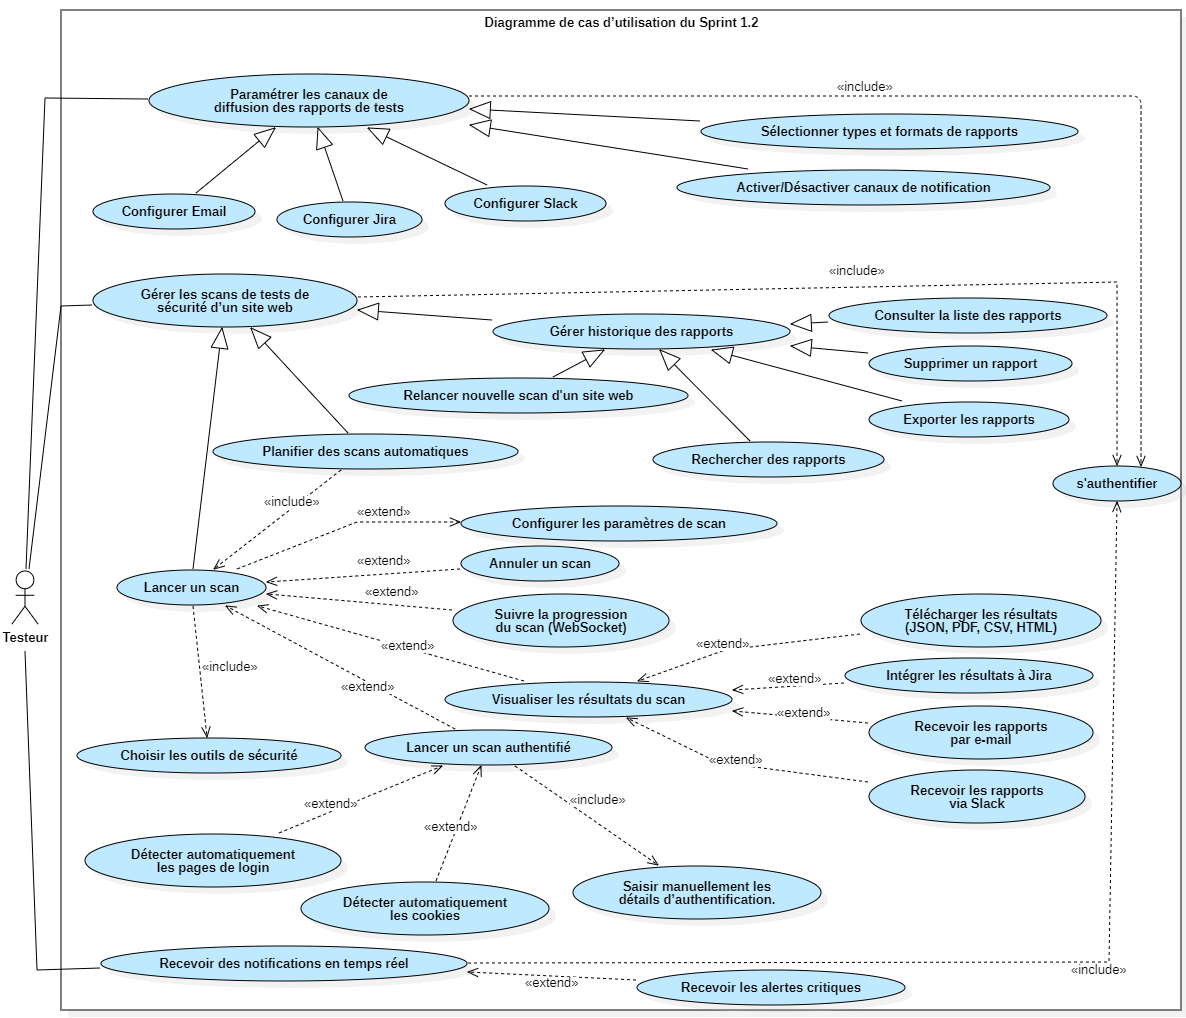
\includegraphics[width=\linewidth]{chapitres/ch3Sp1/section/sprint2/img/LastUseCaseSprint1.2.png}
\caption{Diagramme de cas d’utilisation du sprint 1.2}
\label{fig:caseS2}
\end{figure}
\vspace{-0.6cm}
\subsubsection{Raffinement des cas d’utilisation}
Cette phase d’affinement a permis de clarifier les interactions entre les acteurs et le système, d’identifier les éventuelles dépendances fonctionnelles, et de décomposer les fonctionnalités complexes en sous-cas d’utilisation plus précis.
\begin{enumerate}[label=\alph*), left=-0.1cm]
    \item \textbf{Description textuelle du cas d’utilisation "Choisir les outils de sécurité}\\
        Le tableau ~\ref{tab:tools-select}  présente la description textuelle du cas d’utilisation "Choisir les outils de sécurité".
                  \begin{spacing}{1}
                        \begin{longtable}{|p{0.12\linewidth}|p{0.88\linewidth}|}
                            \caption{Description textuelle du cas d’utilisation : Choisir les outils de sécurité}
                            \label{tab:tools-select}\\
                            \hline
                            \textbf{Titre} & Choisir les outils de sécurité \\
                            \hline
                            \textbf{Acteur} & Testeur \\
                            \hline
                            \textbf{Résumé} & Ce cas d'utilisation permet au testeur de sélectionner les outils qu’il souhaite utiliser pour les futurs scans et enregistre cette configuration pour la réutiliser. \\
                            \hline
                            \textbf{Pré-conditions} & Le testeur est connecté. Les outils disponibles sont listés dynamiquement depuis le backend. \\
                            \hline
                            \textbf{Post-conditions} & Les préférences du testeur sont enregistrées en base de données et réutilisées automatiquement dans les scans suivants. \\
                            \hline
                            \textbf{Scénario nominal} & 
                            \begin{minipage}{\linewidth}
                                \vspace{0.1cm}
                                \begin{enumerate}[label=\arabic*., left=0.1cm]
                                    \item L'utilisateur accède à l’interface de sélection.
                                    \item Il choisit les outils à utiliser via des cases à cocher. 
                                    \item Il valide sa sélection. 
                                    \item Le backend enregistre la configuration. 
                                    \item Un message de confirmation apparaît. 
                                \end{enumerate}
                                \vspace{0.1cm}
                            \end{minipage}\\
                            \hline
                            \textbf{Scénario d’erreur} &
                            \begin{minipage}{\linewidth}
                                \vspace{0.1cm}
                                \begin{itemize}[left=0cm]
                                    \item[\textbullet] \textbf{Étape 3 (Informations incomplètes):}
                                    \begin{itemize}[label=\ding{56}]
                                        \item Si aucun outil n’est sélectionné alors le système affiche un message d’erreur .
                                    \end{itemize}
                        
                                    \item[\textbullet] \textbf{Étape 4 (Erreur d'enregistrement):}
                                    \begin{itemize}[label=\ding{56}]
                                        \item En cas d’échec lors de l’enregistrement des données, le système affiche un message d’erreur "préférences non enregistrées" et invite à réessayer ultérieurement.
                                    \end{itemize}
                                \end{itemize}
                                \vspace{0.1cm}
                            \end{minipage}\\
                            \hline
                        \end{longtable}
                    \end{spacing}
                  \vspace{-0.2cm}
\end{enumerate}




\subsection{Conception du sprint 1.2}
La phase de conception du sprint 1.2 débute par l’élaboration du diagramme de classes, suivi de diagrammes de séquence représentant divers cas d'utilisation. 

\subsubsection{Diagramme de classe du sprint 1.2}
Ce diagramme vise à modéliser les principales entités métier du système, leurs attributs, leurs méthodes ainsi que les relations existantes entre elles.

La figure \ref{fig:classsp1} présente le diagramme de classes correspondant à ce sprint.
\begin{figure}[H]
    \centering
    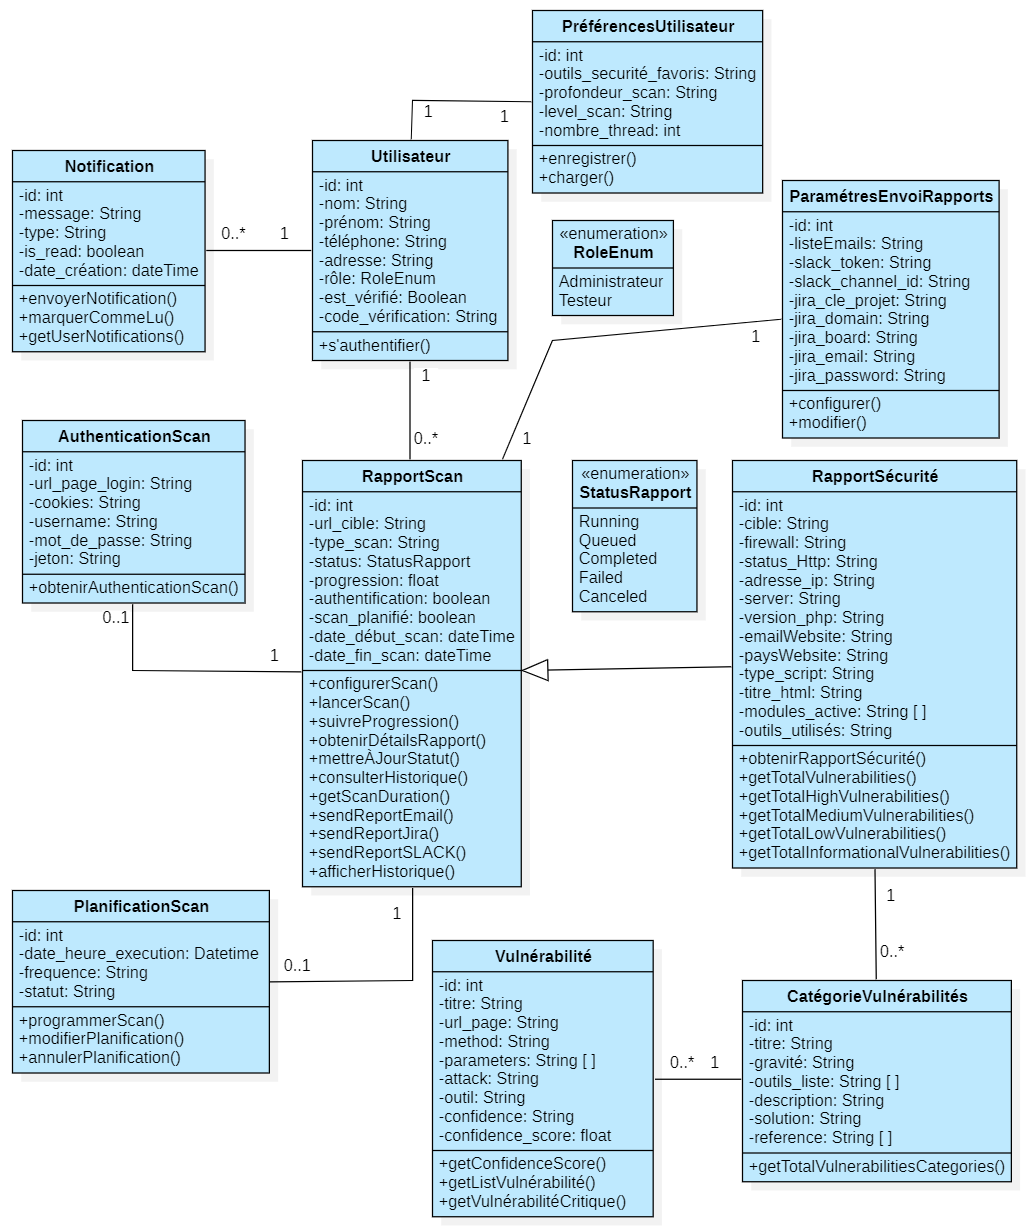
\includegraphics[width=0.9\linewidth]{chapitres/ch3Sp1/section/sprint2/img/classeL1-SP1.2.png}
    \caption{Diagramme de classe du sprint 1.2}
    \label{fig:classsp1}
\end{figure}
\vspace{-0.6cm}
Les principales classes modélisées sont les suivantes :
\begin{itemize}[label=$*$]
    \item \textbf{Utilisateur} : Représente un utilisateur de l’application.
    \item \textbf{PréférencesUtilisateur} : Contient les préférences techniques d’un utilisateur pour les scans (profondeur, niveau, nombre de threads, outils favoris), associée de manière 1-à-1 avec la classe \texttt{Utilisateur}.
    
    \item \textbf{Notification} : Gère les notifications envoyées aux utilisateurs, avec des attributs comme le message, le type et la date de création. Un utilisateur peut recevoir plusieurs notifications.
    
    \item \textbf{ParametresEnvoiRapports} : Stocke les paramètres nécessaires pour l’envoi des rapports (emails, Slack, Jira), incluant les jetons, identifiants et adresses associées à chaque canal de communication.
    
    \item \textbf{RapportScan} : Regroupe les données liées à un scan de sécurité, comme le type de scan, son état (via \texttt{StatusRapport}), la cible, les dates de début/fin, les outils utilisés... Cette classe contient également des méthodes pour configurer, lancer et suivre un scan.
    
    \item \textbf{AuthenticationScan} : Contient les informations nécessaires pour effectuer un scan authentifié (page de login, identifiants, cookies, jetons). Un rapport de scan peut avoir 0 ou 1 configuration d’authentification.
    \item \textbf{RapportSecurite} : Fournit des détails techniques sur l’environnement cible d’un scan : en-têtes HTTP, serveur, version PHP, adresse IP, pays d’hébergement, titre HTML, etc.
    \item \textbf{PlanificationScan} : Permet de planifier l’exécution automatique d’un scan à une date donnée avec une fréquence spécifique. Elle offre des méthodes de gestion comme la mise à jour ou l’annulation d’un scan planifié. Un scan peut être associé à une planification. 
    \item \textbf{Vulnérabilité} : Décrit une vulnérabilité détectée, avec ses détails techniques (type d’attaque, méthode HTTP, paramètres concernés, gravité, score de confiance...) avec des méthodes pour calculer le nombre de vulnérabilités par criticité..
    \item \textbf{CatégorieVulnérabilités} : Catégorise les vulnérabilités détectées selon leur nature, leur niveau de risque, les outils les ayant détectées, la description,  la solution recommandée... Une catégorie peut regrouper plusieurs vulnérabilités.
    \item \textbf{StatusRapport (Énumération)} : Représente l’état d’avancement d’un rapport de scan. Les valeurs possibles sont : \texttt{Running}, \texttt{Queued}, \texttt{Completed}, \texttt{Failed}, et \texttt{Canceled}.
\end{itemize}
Les associations entre classes sont également représentées dans le diagramme, notamment:
\begin{itemize}[label=$-$]
    \item Un \texttt{utilisateur} peut recevoir plusieurs \texttt{notifications}.
    \item Un \texttt{rapport de scan} peut être lié à une ou plusieurs \texttt{vulnérabilités} et appartenir à une \texttt{catégorie} donnée.
    \item Un \texttt{scan} peut être planifié via la classe \texttt{"PlanificationScan"}.
    \item Un \texttt{rapport de sécurité} est généralement associé à un scan donné.
\end{itemize}
Ce diagramme constitue une base essentielle pour la suite du développement, en assurant une structure cohérente et maintenable du code tout au long des itérations agiles.

\subsubsection{Diagramme de séquence de conception}
Les diagrammes de séquence visant à décrire dynamiquement l’enchaînement des interactions entre objets pour différents cas d'utilisation.

\textbf{Diagramme de séquence de conception de cas «Lancer un scan de test sécurité»}:\\
Le diagramme présenté illustre le processus de lancement d’un scan de test de sécurité à travers l'interaction des différents composants du système.
\begin{itemize}[label=$-$]
    \item \textbf{Lancement du scan:} L’utilisateur initie un scan via l’interface. Le backend (FastAPI) reçoit la requête, crée une nouvelle entrée dans la base de données avec le statut \textit{"pending"}, et publie la tâche de scan dans la file RabbitMQ en incluant l'identifiant du scan.
    \item \textbf{Mise en file d’attente:} Si un worker (processus de traitement) est disponible, il récupère la tâche. Si aucun worker n’est libre (file pleine), la tâche est mise en attente. Le statut du scan est alors mis à jour à \textit{"queued"}, une notification d’attente est envoyée via WebSocket, et un message d’attente est affiché à l’utilisateur.
    \item \textbf{Exécution du scan:} Dès qu’un worker devient disponible, le scan passe au statut \textit{"running"}. L’exécution des outils de pentest démarre (en mode multithread via la classe \texttt{GestionnairePentestClass}). Le backend met à jour le pourcentage de progression dans la base de données, et ces informations sont transmises en temps réel à l’interface utilisateur via WebSocket.
    \item \textbf{Détection de vulnérabilités critiques:} Si des vulnérabilités critiques sont identifiées, elles sont envoyées via WebSocket à l’utilisateur en temps réel et affichées immédiatement.
    \item \textbf{Finalisation du scan:} Une fois l’analyse terminée, les résultats et le rapport sont enregistrés dans la base de données. Le statut du scan est mis à jour à \textit{"completed"}, et le rapport final est envoyé à l’utilisateur pour affichage.
\end{itemize}

Ce mécanisme asynchrone, reposant sur RabbitMQ et une architecture multithreadée, permet de gérer plusieurs scans simultanément tout en assurant une communication en temps réel avec l’utilisateur.
\begin{figure}[H]
    \centering
    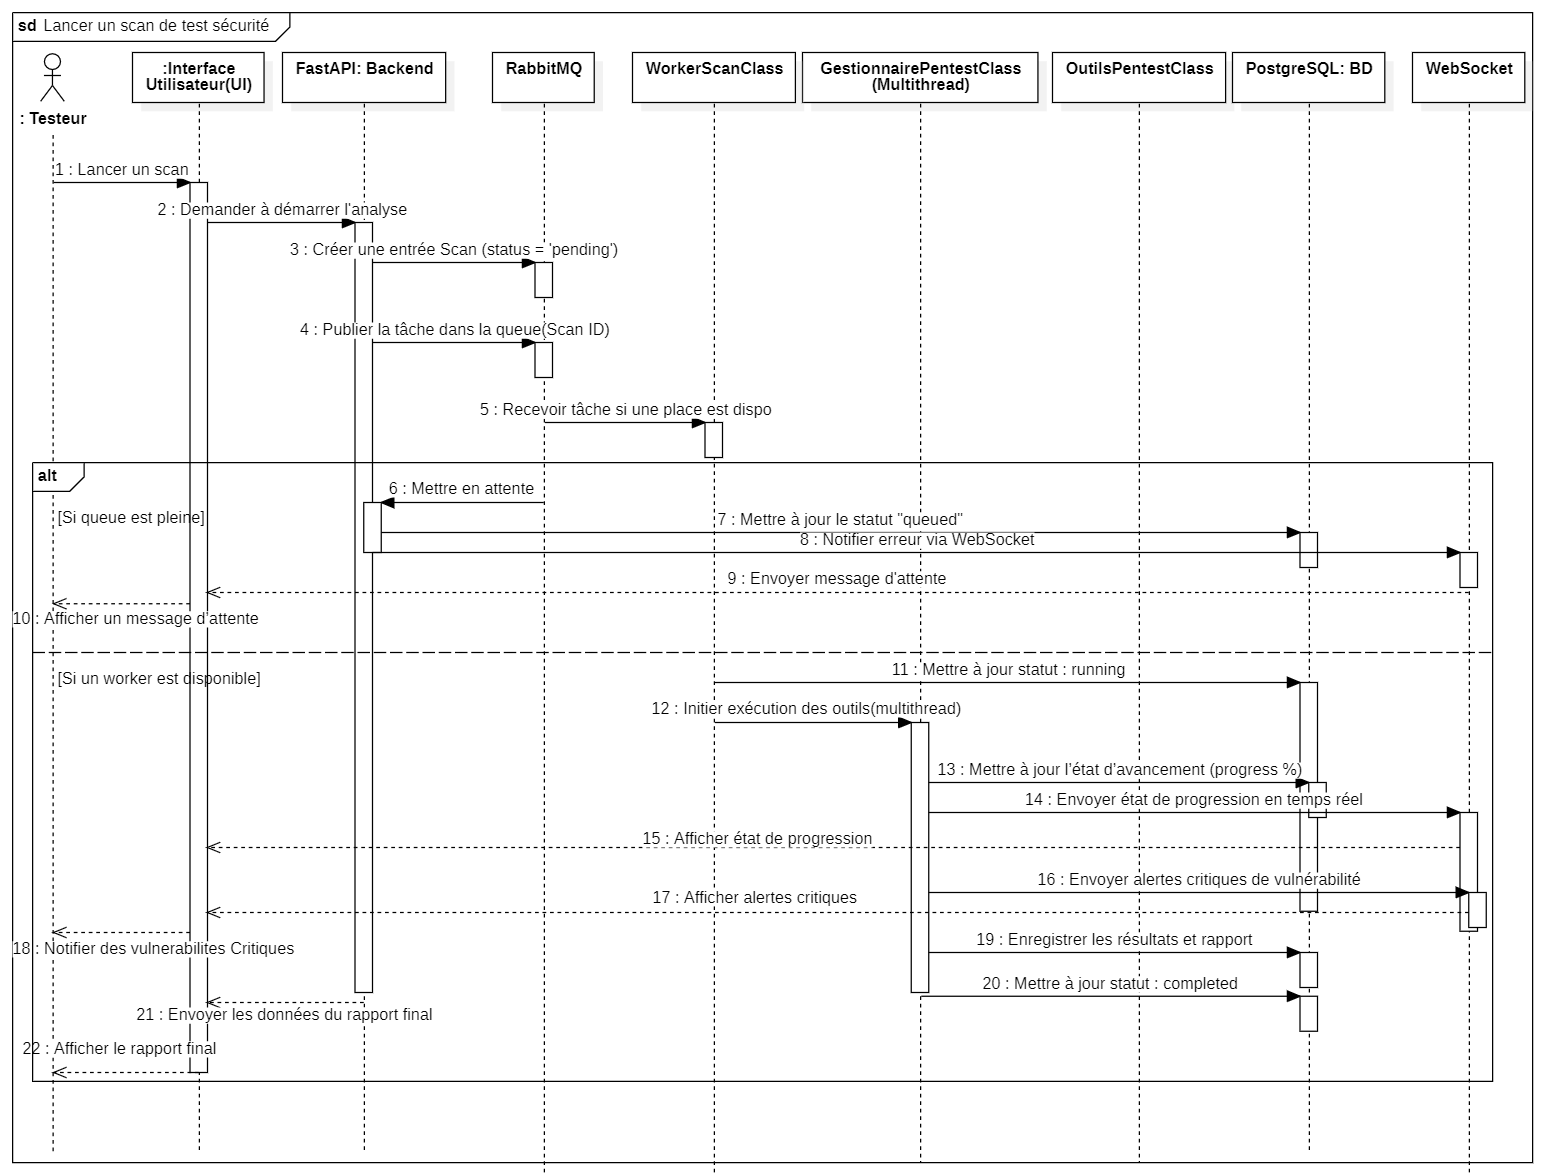
\includegraphics[width=\linewidth]{chapitres/ch3Sp1/section/sprint2/img/seq-lancerSp1.2.png}
    \caption{\centering Diagramme de séquence de conception de cas «Lancer un scan de test sécurité»}
    \label{fig:seq1ScanAnalyse}
\end{figure}
\vspace{-0.6cm}

\subsection{Réalisation du sprint 1.2}
Dans cette section, nous présentons les principales interfaces réalisées au cours du sprint 1.2. 
\begin{itemize}[label=$\bullet$]
    \item \textbf{Interface de configuration des paramètres de scan}:
    La figure \ref{fig:interface_parametres_scan}\footnote{Voir Annexe E, figure \ref{fig:interface_parametres_scan}} illustre l’interface permettant de personnaliser les paramètres d’un scan. Celle-ci permet à l’utilisateur de définir la profondeur de l’analyse, d’activer ou non certains modules (comme le spider ou le scan AJAX), ou encore de choisir des options spécifiques à certains outils.
    
    \item \textbf{Interface de sélection des outils de sécurité}:
    La figure \ref{fig:interface_selection_outils} présente l’écran dédié à la sélection des outils de sécurité. Cette interface propose une liste de cases à cocher pour activer ou désactiver les outils disponibles, accompagnée de boutons «Tout sélectionner» et «Tout désélectionner». Les préférences de l’utilisateur sont sauvegardées pour les réutiliser dans les futurs scans.
     \begin{figure}[H]
        \centering
        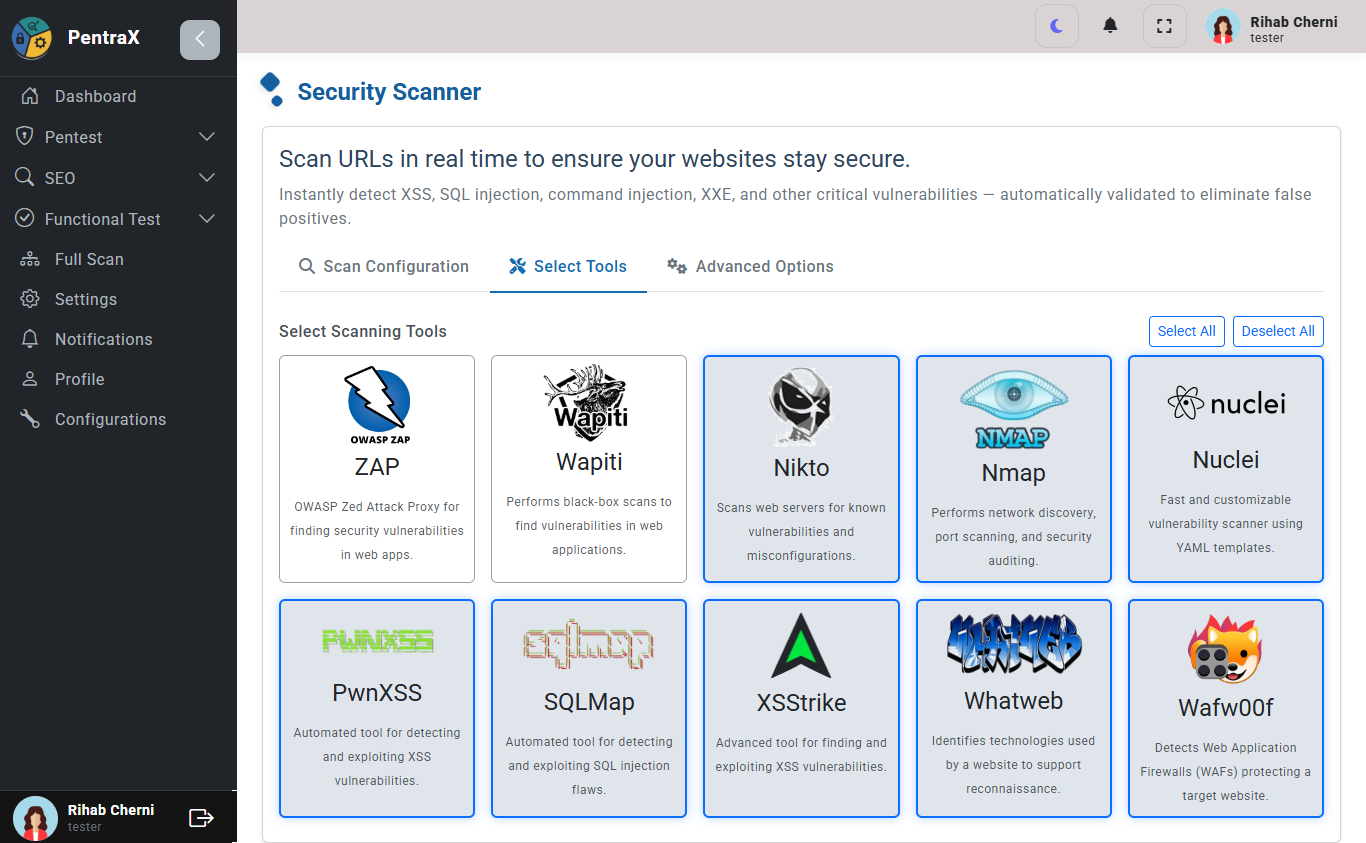
\includegraphics[width=\textwidth]{chapitres/ch3Sp1/section/sprint2/img/interface/tools.png}
        \caption{Interface de sélection des outils de sécurité}
        \label{fig:interface_selection_outils}
    \end{figure}
    \vspace{-0.2cm}
    \item \textbf{Interface utilisateur pour le lancement de scans, avec ou sans authentification} :\\
        La figure \ref{fig:interface_lancement_scan} illustre le formulaire principal de lancement d’un test de sécurité. L’utilisateur y renseigne l’URL de la cible, choisit les outils à utiliser, configure les paramètres du scan, puis lance l’analyse via un bouton dédié.

        Cette interface propose également une section dédiée à l’authentification, activable via des boutons radio. En fonction du type sélectionné, les champs correspondants s’affichent dynamiquement : identifiants (nom d’utilisateur et mot de passe), jetons d’accès (tokens), ou cookies de session. Cette fonctionnalité est essentielle pour analyser les zones protégées d’une application web. Pour plus de détails sur le lancement des scans de sécurité, la gestion des paramètres d’authentification et la configuration des outils, voir l’annexe C\footnote{Voir Annexe C: Automatisation des outils de pentesting}.
        \begin{figure}[H]
            \centering
            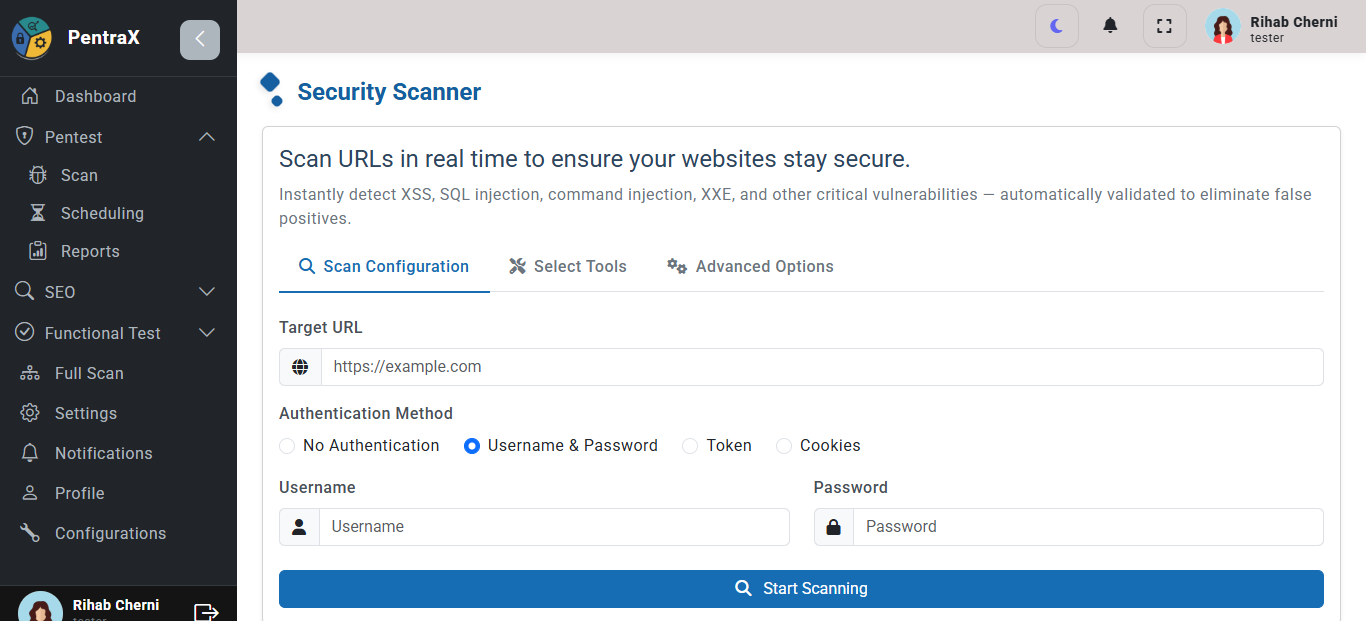
\includegraphics[width=\textwidth]{chapitres/ch3Sp1/section/sprint2/img/interface/start-sca.PNG}
            \caption{Interface de lancement de scan avec ou sans authentification}
            \label{fig:interface_lancement_scan}
        \end{figure}
        \vspace{-0.2cm}
    \item \textbf{Interface de suivi en temps réel des scans}: Comme illustré dans la figure \ref{fig:interface_suivi_ws}\footnote{Voir Annexe E, figure \ref{fig:interface_suivi_ws}}, cette interface permet de suivre l’évolution du scan en temps réel grâce à l’intégration des WebSockets, avec un indicateur de progression affiché de 0 à 100\,\%.    
    \item \textbf{Interface de visualisation des résultats}:
    La figure \ref{fig:interface_resultats_scan} montre l’écran de consultation des vulnérabilités détectées. Des filtres par type, gravité ou outil sont proposés pour affiner l’analyse, et chaque vulnérabilité est accompagnée d’un résumé, de son risque, de sa source et d’une suggestion de correction.
        \begin{figure}[H]
            \centering
            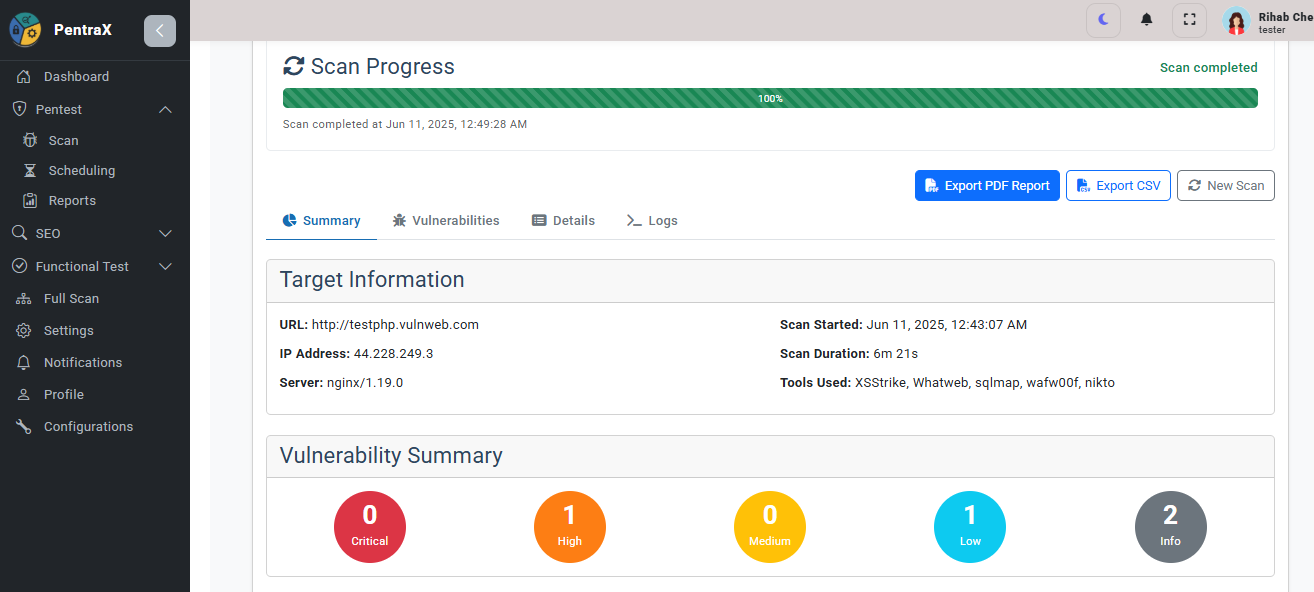
\includegraphics[width=\textwidth]{chapitres/ch3Sp1/section/sprint2/img/interface/res1.PNG}
            \caption{\centering Interface de visualisation des résultats de scan (premier onglet : statistiques et détails techniques)}
            \label{fig:interface_resultats_scan}
        \end{figure}
        \vspace{-0.2cm}
    \item \textbf{Interface de l’historique des scans}:
    L’interface illustrée par la figure \ref{fig:interface_historique_scans}\footnote{Voir Annexe E, figure \ref{fig:interface_historique_scans}} permet d’accéder aux rapports précédemment générés. Une table paginée présente les scans enregistrés, accompagnée de filtres, d’un champ de recherche, et d’une option de suppression.
    
    \item \textbf{Interface de téléchargement des rapports}:
    Comme présenté dans la figure \ref{fig:interface_export_rapports}\footnote{Voir Annexe E, figure \ref{fig:interface_export_rapports}}, cette interface permet de télécharger les rapports aux formats JSON, PDF ou CSV, selon les besoins de l’utilisateur.


    \item \textbf{Interface pour le paramétrage des canaux de diffusion} : La figure \ref{fig:interface_parametrage_canaux}\footnote{Voir Annexe E, figure \ref{fig:interface_parametrage_canaux}} illustre l’interface dédiée à la configuration détaillée des canaux de diffusion des rapports. Elle permet à l’utilisateur de spécifier, pour chaque type de test (sécurité, SEO, fonctionnel), les canaux de notification souhaités (Slack, Jira, Email), le format du rapport associé (PDF, HTML, JSON). Des champs dynamiques permettent d’ajouter plusieurs destinataires e-mail et d’entrer des clés API sécurisées pour Slack et Jira. Cette interface vise à centraliser et automatiser la diffusion ciblée des rapports vers les bons interlocuteurs.

    \item \textbf{Interface d’intégration Jira}:
    La figure \ref{fig:interface_jira_integration}\footnote{Voir Annexe E, figure \ref{fig:interface_jira_integration}} illustre la fonctionnalité d’envoi des vulnérabilités détectées directement vers Jira pour créer automatiquement des tickets. Un aperçu des tickets créés est également affiché.
    
    \item \textbf{Interface de notification Slack et e-mail}:
    Les figures \ref{fig:interface_slack_notification} et \ref{fig:interface_email_notification}\footnote{Voir Annexe E, figures \ref{fig:interface_slack_notification} et \ref{fig:interface_email_notification}} présentent respectivement l’envoi automatique des rapports via Slack et e-mail. Ces notifications sont déclenchées à la fin du scan, contenant un résumé des vulnérabilités et un lien vers le rapport complet.
    
    \item \textbf{Interface de planification automatique des scans}:  
    La figure \ref{fig:interface_planification_scan}\footnote{Voir Annexe E, figure \ref{fig:interface_planification_scan}} illustre l’écran de planification permettant à l’utilisateur de définir des scans récurrents. Il peut spécifier la fréquence (quotidienne, hebdomadaire, mensuelle), l’heure d’exécution, la cible concernée et les paramètres associés. Une liste des tâches planifiées est également visible et modifiable.
    
    \item \textbf{Interface de gestion centralisée des notifications}: La figure \ref{fig:interface_notifications_config}\footnote{Voir Annexe E, figure \ref{fig:interface_notifications_config}} présente une interface unifiée permettant à l’utilisateur d’activer et de configurer les canaux de diffusion des rapports vers Jira, Slack et l’e-mail. L’interface offre des options pour sélectionner les canaux souhaités, saisir les identifiants API (Slack, Jira ou les adresses e-mail), et choisir les formats (HTML, PDF, JSON) ainsi que les types de rapports à transmettre (sécurité, fonctionnel, SEO).
\end{itemize}



















% \section{Sprint 1.2 : Automatisation des tests de sécurité et gestion des utilisateurs (25 jours)}
% Le second sprint de cette première livraison a été axé sur des fonctionnalités plus complexes liées à la sécurité et à l’interaction utilisateur.
% \begin{itemize}[label=$-$]
%     \item Développement du module de gestion des scans de tests de sécurité ;
%     \item Gestion des utilisateurs ;
%     \item Implémentation des notifications en temps réel.
% \end{itemize}

% \subsection{Gestion des scans de tests de sécurité}
% Ce module permet d’analyser automatiquement les vulnérabilités potentielles dans les sites web soumis par les utilisateurs. Il inclut :

% L’intégration d’un moteur d’analyse de sécurité (comme OWASP ZAP ou une API interne) ;

% Le lancement et le suivi des scans ;

% L’affichage des résultats (failles détectées, niveau de risque, etc.) ;

% L’archivage des rapports pour consultation ultérieure.

% Cette automatisation renforce la valeur ajoutée du projet en permettant une surveillance proactive.

% \subsection{Gestion des utilisateurs}
% Ce sous-module permet l’administration des comptes utilisateurs. Les fonctionnalités développées comprennent :

% La visualisation de la liste des utilisateurs ;

% La modification ou suppression de comptes ;

% L’attribution de rôles ou de privilèges selon les besoins du système.

% Cette partie assure un meilleur contrôle sur les accès à la plateforme.

% \subsection{Notifications en temps réel}
% Le système de notifications permet d’informer instantanément les utilisateurs des événements importants, comme :

% Le début ou la fin d’un scan ;

% La réception d’un rapport de vulnérabilités ;

% Des alertes système ou des changements de statut.

% Cette fonctionnalité a été réalisée à l’aide de WebSockets (ou d’une alternative comme Pusher ou Firebase selon la stack choisie), assurant une communication fluide et réactive.


%  \section{Backlog du sprint 1.2}  
% Dans cette section, nous présentons le backlog du sprint 1.2, tel qu'illustré dans le tableau \ref{tab:backlogS22}.
Ce backlog détaille les besoins sélectionnées pour ce sprint, accompagnées de leurs tâches associées, priorités, risques et estimations en jours.
\begin{landscape}
    \renewcommand{\arraystretch}{1.3}
    \begin{spacing}{0.94}
        \begin{longtable}{|p{0.6cm}|p{2.6cm}|p{4.9cm}|p{0.97cm}|p{8.6cm}|p{0.35cm}|p{0.35cm}|p{1.6cm}|}
            \caption{Backlog du sprint 1.2} \label{tab:backlogS22} \\\hline
            \rowcolor{gray!20}
            \textbf{\small ID US} & 
            \multicolumn{1}{c|}{\textbf{\small User Story}} & 
            \multicolumn{1}{c|}{\textbf{\small Description}} & 
            \textbf{\small ID tâche}& 
            \multicolumn{1}{c|}{\textbf{\small Tâches}} & 
            \multicolumn{1}{c|}{\textbf{\small Priorité}} & 
            \multicolumn{1}{c|}{\textbf{\small Risques}} & 
            \textbf{\fontsize{9}{11}\selectfont Estimation (Jours)}\\\hline
            % ----------- SCANS DE SÉCURITÉ ------------------
			\rowcolor{blue!20}
            \multicolumn{8}{|c|}{\textbf{EPIC 4: Gestion des scans de tests de sécurité d’un site web}} \\\hline
            
            4.1 & Configurer les paramètres de scan selon les besoins. & En tant que testeur, je veux personnaliser les paramètres de scan pour adapter les analyses aux besoins spécifiques. 
            & 4.1.A \newline\vspace{0.5cm} 4.1.B &
            - Développer une interface pour configurer les paramètres de scan. \newline
            - Permettre à l’utilisateur de choisir la profondeur des scans. & Moyenne & Moyenne & 1/2\\ \hline

           4.2 & Sélectionner les outils de sécurité à utiliser pour l’analyse.
            & En tant que testeur, je veux choisir les outils à utiliser afin d’adapter l’analyse aux besoins de la cible, enregistrer mes préférences et les réutiliser lors des scans suivants.
             & 4.2.A \newline\vspace{1.9cm} 4.2.B&
            - Développer une interface avec des cases à cocher permettant de sélectionner les outils souhaités avant le lancement d’un scan avec une sélection multiple et des boutons « Tout sélectionner » / « Tout désélectionner ».\newline
            - Enregistrer les outils préférés de chaque utilisateur dans la base de données et les recharger automatiquement pour les scans suivants.
            & Élevée  & Élevée  & 1\\ \hline
            
            4.3 & Lancer un scan de test de sécurité. & En tant que testeur, je veux initier un scan de test de sécurité sur une cible pour identifier ses vulnérabilités. 
            & 
            4.3.A \newline\vspace{1cm} 
            4.3.B\newline\vspace{0.9cm} 
            4.3.C\newline\vspace{0.5cm} 
            4.3.D\newline\vspace{0.5cm} 
            4.3.E\newline\vspace{0.5cm} 
            4.3.F\newline\vspace{0.5cm} 
            4.3.G&
            - Développer une interface de lancement de scan avec champ URL de la cible à tester, les outils, paramètres de scan et bouton "Lancer".\newline
            - Corriger l'automatisation des outils existants \textbf{ZAP} et \textbf{Wapiti} en vérifiant leur configuration et optimisant les paramètres de détection.\newline
            - Intégrer et automatiser l’exécution d’outils spécialisés tels que SQLMap, Nuclei, Nmap...\newline
            - Utiliser le multithreading pour exécuter les outils en parallèle.\newline
            - Unifier les formats de sortie pour générer un rapport commun.\newline
            - Créer une base de données des vulnérabilités détectées.\newline
            - Générer un rapport JSON unifié via un modèle d’agrégation et de comparaison.
            & Élevée & Moyenne & 1 \\ \hline
            
            4.4 & Lancer un scan de sécurité avec authentification dynamique. 
                & En tant que testeur, je souhaite initier un scan authentifié afin d’identifier les vulnérabilités présentes dans les zones protégées.  & 4.4.A \newline\vspace{0.5cm} 4.4.B  & 
                - Intégrer l’authentification dynamique pour chaque outil. \newline
                - Tester les mécanismes d’authentification pour chaque outil (cookies, jetons, mots de passe). & Élevée & Moyenne &3 \\ \hline
            
            4.5 & Planifier des scans  de test sécurité automatiques. 
                & En tant que testeur, je veux définir une planification automatique des scans pour assurer une surveillance régulière. & 4.5.A \newline\vspace{0.5cm} 4.5.B  &
                - Créer une interface de planification pour automatiser les scans. \newline
                - Tester le bon déroulement des scans planifiés. & Élevée & Moyenne & 1 \\ \hline
                
            4.6 & Suivre la progression du scan en temps réel via WebSocket. 
                & En tant que testeur, je veux visualiser en temps réel l’évolution des scans pour suivre leur progression.
                & 4.6.A \newline 4.6.B &
                - Intégrer WebSocket pour suivre la progression. \newline
                - Mettre à jour l'interface utilisateur avec des informations en temps réel.  & Élevée & Moyenne & 1 \\ \hline            
            4.7 & Visualiser les résultats des scans. 
                    & En tant que testeur, je peux consulter les résultats afin d'analyser la sécurité de l'application. 
                    & 4.7.A \newline\vspace{0.5cm} 4.7.B
                    & 
                    - Implémenter une interface pour visualiser les résultats des scans. \newline
                    - Fournir des options de filtrage pour faciliter l'analyse des résultats. 
                    & Élevée & Basse & 2 \\
                \hline
            4.8 & Accéder à l’historique des scans précédents. 
                    & En tant que testeur, je dois accéder aux rapports des anciens scans pour suivre l'évolution des vulnérabilités et conserver une trace des analyses précédentes.
                    & 4.8.A 
                    \newline 4.8.B
                    \newline\vspace{0.5cm} 4.8.C
                    \newline 4.8.D
                    \newline\vspace{0.4cm} 4.8.E
                    \newline\vspace{0.5cm} 4.8.F
                    \newline\vspace{0.cm} 4.8.G
                    & 
                     - Afficher les historiques de scans.\newline
                     - Ajouter une pagination pour naviguer entre les pages de résultats.\newline
                     - Ajouter des filtres (par type, outil, gravité...). \newline
                     - Implémenter une barre de recherche pour retrouver un scan précis.\newline
                     - Ajouter une option de suppression pour chaque rapport.\newline
                     - Permettre l'accès aux détails d’un scan : liste des vulnérabilités par outil et les logs associés à chaque scan.\newline
                     - Afficher un résumé global du scan accompagné de la liste complète des vulnérabilités détectées pour chaque scan.
                    & Moyenne & Basse & 1 \\
                \hline
                4.9 & Télécharger les rapports aux formats JSON, PDF et CSV. 
                    & En tant que testeur, je dois télécharger les rapports sous différents formats pour faciliter leur traitement et archivage. 
                    & 4.9.A \newline\vspace{0.5cm} 4.9.B
                    & 
                    - Développer des options d'exportation pour les rapports. \newline
                    - Ajouter des boutons pour télécharger les rapports en formats JSON, PDF et CSV.
                    & Moyenne & Moyenne & 1 \\
                \hline
                4.10 & Intégrer et visualiser les rapports via Jira. 
                    & En tant que testeur, je dois intégrer les résultats dans Jira pour créer des tickets et assurer un suivi structuré des incidents détectés. 
                    & 4.10.A \newline\vspace{0.5cm} 4.10.B
                    & 
                    - Créer une intégration avec Jira pour la création automatique de tickets. \newline
                    - Visualiser les résultats dans des dashboards Jira.
                    & Élevée & Élevée & 3/2 \\
                \hline
                4.11 & Accéder aux rapports via Slack. 
                    & En tant que testeur, je dois recevoir les rapports via Slack pour une communication rapide au sein de l'équipe. 
                    & 4.11.A \newline\vspace{0.5cm} 4.11.B
                    & 
                    - Mettre en place une intégration avec Slack pour envoyer les rapports. \newline
                    - Ajouter des notifications Slack pour chaque scan terminé.
                    & Moyenne & Basse & 3/2 \\
                \hline
                4.12 & Recevoir les rapports directement par e-mail. 
                    & En tant que testeur, je dois recevoir automatiquement les rapports par e-mail pour assurer leur disponibilité hors plateforme. 
                    & 4.12.A \newline\vspace{0.5cm}4.12.B
                    & 
                    - Configurer l'envoi automatique de rapports par e-mail. \newline
                    - Ajouter un modèle d'e-mail pour l'envoi des rapports.
                    & Moyenne & Basse & 3/2 \\
                \hline
                4.13 & Détecter automatiquement les pages de login, en excluant les pages d’inscription. 
                    & En tant que testeur, je souhaite que le système identifie automatiquement les pages d’authentification d’un site pour configurer correctement les scans authentifiés. 
                    & 4.13.A \newline\vspace{0.5cm} 4.13.B
                    & 
                    - Analyser le code HTML des pages pour détecter les formulaires de connexion.\newline
                    - Mettre en place des règles pour exclure les pages d’inscription et les pages non pertinentes.
                    & Élevée & Moyenne & 2 \\
                \hline
                4.14 & Annuler un scan de sécurité en cours. 
                    & En tant que testeur, je souhaite pouvoir annuler un scan de sécurité en cours d'exécution afin d’arrêter une analyse inutile ou incorrectement configurée.
                    & 4.14.A \newline\vspace{0.5cm} 4.14.B
                    & 
                    - Ajouter un bouton "Annuler" dans l'interface de suivi en temps réel du scan.\newline
                    - Implémenter la logique backend pour interrompre proprement l'exécution des outils lancés (thread/process/containers).
                    & Élevée & Moyenne & 2 \\
                \hline
                4.14 & Relancer un scan à partir de la configuration précédente.
                & En tant que testeur, je souhaite relancer facilement un scan de sécurité en utilisant les paramètres d’un ancien scan pour gagner du temps et assurer la reproductibilité des tests.
                & 4.14.A \newline\vspace{0.5cm} 4.14.B 
                &
                - Permettre la duplication d’un scan depuis l’historique avec récupération automatique de la configuration (outils, paramètres, cible, type d’authentification, etc.). \newline
                - Développer une interface "Relancer ce scan" accessible depuis les détails d’un scan précédent. \newline
                & Moyenne & Moyenne & 1 \\
            \hline

        % ----------- Notifications ------------------
           \rowcolor{blue!20}
           \multicolumn{8}{|c|}{\textbf{EPIC 9: Notifications en temps réel}} \\\hline
            9.1 & Être notifié des résultats pendant l’exécution des scans. 
                & En tant que testeur, je dois recevoir des notifications immédiates pour suivre l'état des scans et détecter rapidement les incidents. 
                & 9.1.A \newline\vspace{0.5cm} 9.1.B 
                &
                - Configurer le système de notifications en temps réel. \newline
                - Tester l'envoi de notifications pendant l'exécution des scans. 
                & Élevée & Basse & 1 \\ \hline
            9.2 & Envoyer des alertes pour les vulnérabilités critiques. 
                & En tant que testeur, je dois recevoir des alertes spécifiques pour les vulnérabilités critiques afin de pouvoir réagir rapidement. 
                & 9.2.A \newline\vspace{0.5cm} 9.2.B 
                &
                - Définir les critères de vulnérabilités critiques pour l'envoi d'alertes. \newline
                - Automatiser l'envoi des alertes en fonction de la gravité des vulnérabilités détectées. 
                & Élevée & Élevée & 1 \\ \hline
            \hline   
        \rowcolor{blue!20}
           \multicolumn{8}{|c|}{\textbf{EPIC 10: Paramétrage des canaux de diffusion des rapports de tests}} \\\hline
                10.1 & Définir les identifiants et jetons d’accès pour Slack. 
                & En tant que testeur, je veux configurer les identifiants d’accès Slack pour activer l’envoi automatique des rapports dans les canaux de l’équipe.
                & 10.1.A \newline\vspace{0.5cm}10.1.B
                & - Ajouter un formulaire de saisie des tokens Slack.\newline - Tester l’envoi automatisé d’un rapport via Slack.
                & Élevée & Moyenne & 1/2\\\hline
                
                10.2 & Saisir les adresses e-mail des destinataires. 
                & En tant qu’utilisateur, je veux définir les adresses email des destinataires pour permettre la diffusion automatique des rapports.
                & 10.2.A \newline\vspace{0.5cm}10.2.B
                & - Créer une interface de configuration des adresses e-mail.\newline - Tester l’envoi de rapports PDF par e-mail.
                & Moyenne & Faible & 1/2\\\hline
                
                10.3 & Configurer les paramètres d’intégration Jira. 
                & En tant qu’administrateur, je veux paramétrer l’URL, l’ID projet et les clés API Jira pour permettre la création automatisée de tickets avec les résultats de scan.
                & 10.3.A \newline\vspace{0.5cm}10.3.B
                & - Développer une interface de saisie des paramètres Jira.\newline - Tester l’intégration avec la création d’un ticket depuis un rapport.
                & Élevée & Moyenne & 1/2\\\hline
                
                10.4 & Sélectionner les types et formats de rapports à envoyer. 
                & En tant qu’utilisateur, je souhaite choisir quels types (sécurité, fonctionnel, SEO) et quels formats (HTML, PDF, JSON) de rapports seront transmis.
                & 10.4.A \newline\vspace{0.5cm}10.4.B
                & - Implémenter une interface pour sélectionner les types et formats de rapport.\newline - Tester l’envoi avec les différentes combinaisons sélectionnées.
                & Moyenne & Moyenne & 1/4\\\hline
                
                10.5 & Activer ou désactiver les canaux de notification. 
                & En tant qu’utilisateur, je veux activer ou désactiver les notifications Slack, Email ou Jira selon mes préférences.
                & 10.5.A
                & - Ajouter des boutons d’activation/désactivation pour chaque canal.\newline
                & Faible & Faible & 1/4\\\hline
                

            \rowcolor{gray!20}
			\multicolumn{7}{|c|}{TOTAL} &  24 (Jours)\\
            \hline 
        \end{longtable}
    \end{spacing}
    \vspace{-0.1cm}
\end{landscape}



%     \section{Analyse du sprint 1.2}
%     Nous entamons à présent la phase d’analyse du sprint 1.2. Cette section présente le diagramme de cas d’utilisation correspondant aux fonctionnalités ciblées durant ce sprint, accompagné de descriptions textuelles détaillées pour certains cas d’usage.

\subsubsection{Diagramme de cas d’utilisation du sprint 1.2}

La figure \ref{fig:caseS2} illustre le diagramme de cas d’utilisation raffiné du sprint 1.2. Il met en avant les différents cas d’usage planifiés pour ce sprint, en mettant l’accent sur les interactions entre les utilisateurs et les composants du système.

\begin{figure}[H]
\centering
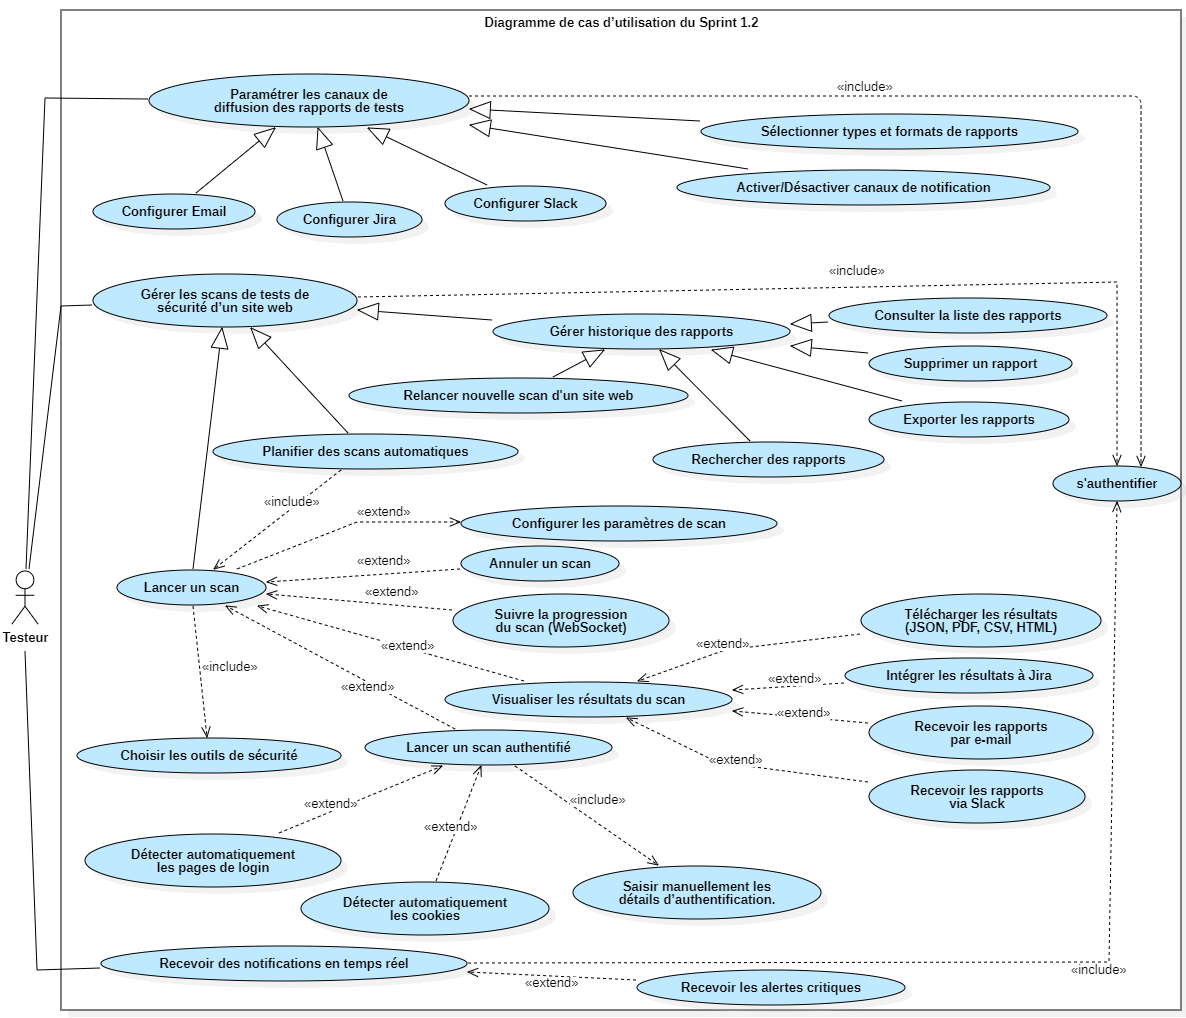
\includegraphics[width=\linewidth]{chapitres/ch3Sp1/section/sprint2/img/LastUseCaseSprint1.2.png}
\caption{Diagramme de cas d’utilisation du sprint 1.2}
\label{fig:caseS2}
\end{figure}
\vspace{-0.6cm}
\subsubsection{Raffinement des cas d’utilisation}
Cette phase d’affinement a permis de clarifier les interactions entre les acteurs et le système, d’identifier les éventuelles dépendances fonctionnelles, et de décomposer les fonctionnalités complexes en sous-cas d’utilisation plus précis.
\begin{enumerate}[label=\alph*), left=-0.1cm]
    \item \textbf{Description textuelle du cas d’utilisation "Choisir les outils de sécurité}\\
        Le tableau ~\ref{tab:tools-select}  présente la description textuelle du cas d’utilisation "Choisir les outils de sécurité".
                  \begin{spacing}{1}
                        \begin{longtable}{|p{0.12\linewidth}|p{0.88\linewidth}|}
                            \caption{Description textuelle du cas d’utilisation : Choisir les outils de sécurité}
                            \label{tab:tools-select}\\
                            \hline
                            \textbf{Titre} & Choisir les outils de sécurité \\
                            \hline
                            \textbf{Acteur} & Testeur \\
                            \hline
                            \textbf{Résumé} & Ce cas d'utilisation permet au testeur de sélectionner les outils qu’il souhaite utiliser pour les futurs scans et enregistre cette configuration pour la réutiliser. \\
                            \hline
                            \textbf{Pré-conditions} & Le testeur est connecté. Les outils disponibles sont listés dynamiquement depuis le backend. \\
                            \hline
                            \textbf{Post-conditions} & Les préférences du testeur sont enregistrées en base de données et réutilisées automatiquement dans les scans suivants. \\
                            \hline
                            \textbf{Scénario nominal} & 
                            \begin{minipage}{\linewidth}
                                \vspace{0.1cm}
                                \begin{enumerate}[label=\arabic*., left=0.1cm]
                                    \item L'utilisateur accède à l’interface de sélection.
                                    \item Il choisit les outils à utiliser via des cases à cocher. 
                                    \item Il valide sa sélection. 
                                    \item Le backend enregistre la configuration. 
                                    \item Un message de confirmation apparaît. 
                                \end{enumerate}
                                \vspace{0.1cm}
                            \end{minipage}\\
                            \hline
                            \textbf{Scénario d’erreur} &
                            \begin{minipage}{\linewidth}
                                \vspace{0.1cm}
                                \begin{itemize}[left=0cm]
                                    \item[\textbullet] \textbf{Étape 3 (Informations incomplètes):}
                                    \begin{itemize}[label=\ding{56}]
                                        \item Si aucun outil n’est sélectionné alors le système affiche un message d’erreur .
                                    \end{itemize}
                        
                                    \item[\textbullet] \textbf{Étape 4 (Erreur d'enregistrement):}
                                    \begin{itemize}[label=\ding{56}]
                                        \item En cas d’échec lors de l’enregistrement des données, le système affiche un message d’erreur "préférences non enregistrées" et invite à réessayer ultérieurement.
                                    \end{itemize}
                                \end{itemize}
                                \vspace{0.1cm}
                            \end{minipage}\\
                            \hline
                        \end{longtable}
                    \end{spacing}
                  \vspace{-0.2cm}
\end{enumerate}




%     \section{Conception du sprint 1.2}
%     La phase de conception du sprint 1.2 débute par l’élaboration du diagramme de classes, suivi de diagrammes de séquence représentant divers cas d'utilisation. 

\subsubsection{Diagramme de classe du sprint 1.2}
Ce diagramme vise à modéliser les principales entités métier du système, leurs attributs, leurs méthodes ainsi que les relations existantes entre elles.

La figure \ref{fig:classsp1} présente le diagramme de classes correspondant à ce sprint.
\begin{figure}[H]
    \centering
    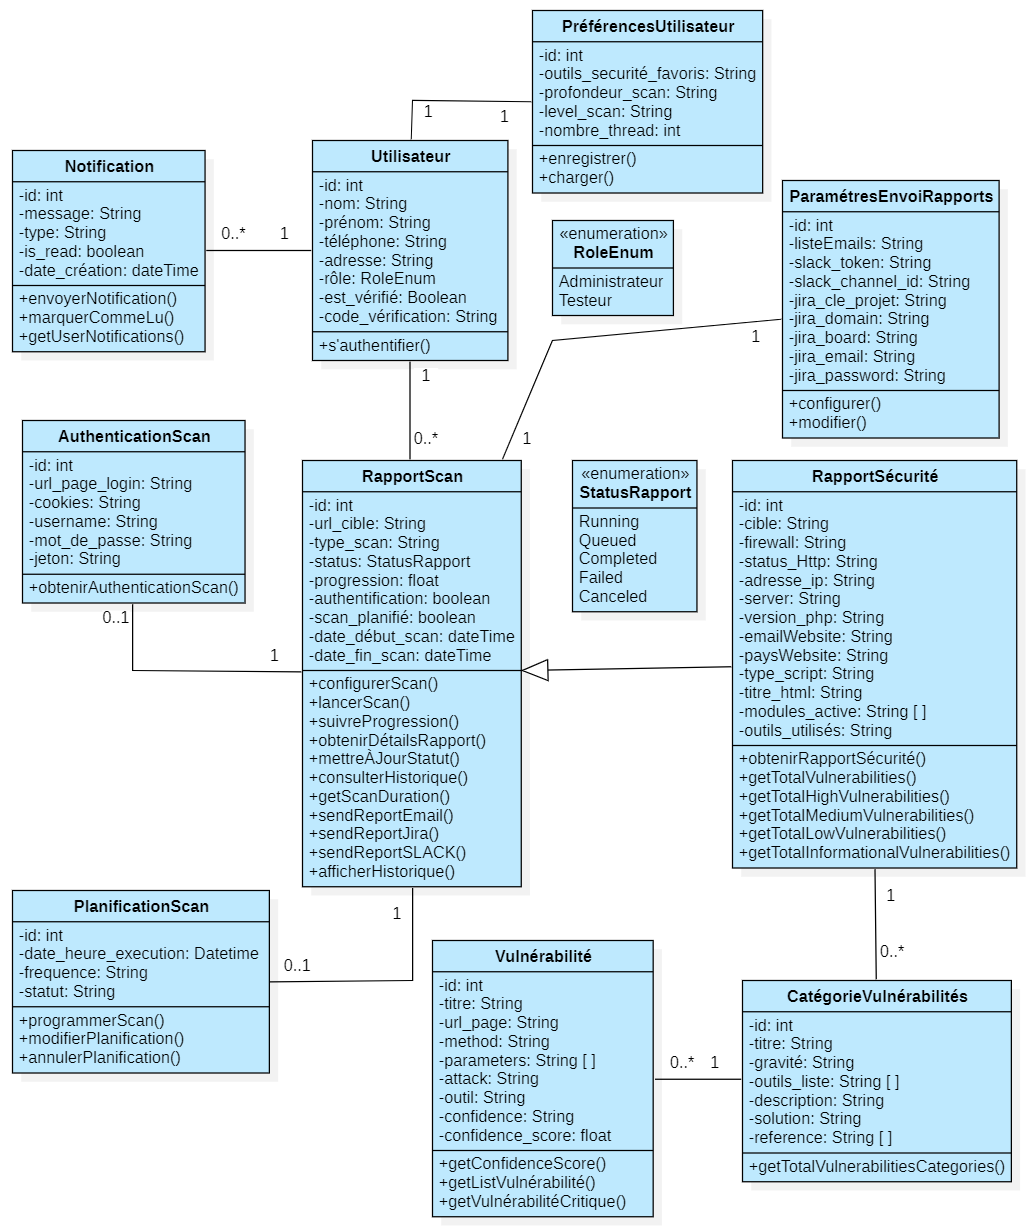
\includegraphics[width=0.9\linewidth]{chapitres/ch3Sp1/section/sprint2/img/classeL1-SP1.2.png}
    \caption{Diagramme de classe du sprint 1.2}
    \label{fig:classsp1}
\end{figure}
\vspace{-0.6cm}
Les principales classes modélisées sont les suivantes :
\begin{itemize}[label=$*$]
    \item \textbf{Utilisateur} : Représente un utilisateur de l’application.
    \item \textbf{PréférencesUtilisateur} : Contient les préférences techniques d’un utilisateur pour les scans (profondeur, niveau, nombre de threads, outils favoris), associée de manière 1-à-1 avec la classe \texttt{Utilisateur}.
    
    \item \textbf{Notification} : Gère les notifications envoyées aux utilisateurs, avec des attributs comme le message, le type et la date de création. Un utilisateur peut recevoir plusieurs notifications.
    
    \item \textbf{ParametresEnvoiRapports} : Stocke les paramètres nécessaires pour l’envoi des rapports (emails, Slack, Jira), incluant les jetons, identifiants et adresses associées à chaque canal de communication.
    
    \item \textbf{RapportScan} : Regroupe les données liées à un scan de sécurité, comme le type de scan, son état (via \texttt{StatusRapport}), la cible, les dates de début/fin, les outils utilisés... Cette classe contient également des méthodes pour configurer, lancer et suivre un scan.
    
    \item \textbf{AuthenticationScan} : Contient les informations nécessaires pour effectuer un scan authentifié (page de login, identifiants, cookies, jetons). Un rapport de scan peut avoir 0 ou 1 configuration d’authentification.
    \item \textbf{RapportSecurite} : Fournit des détails techniques sur l’environnement cible d’un scan : en-têtes HTTP, serveur, version PHP, adresse IP, pays d’hébergement, titre HTML, etc.
    \item \textbf{PlanificationScan} : Permet de planifier l’exécution automatique d’un scan à une date donnée avec une fréquence spécifique. Elle offre des méthodes de gestion comme la mise à jour ou l’annulation d’un scan planifié. Un scan peut être associé à une planification. 
    \item \textbf{Vulnérabilité} : Décrit une vulnérabilité détectée, avec ses détails techniques (type d’attaque, méthode HTTP, paramètres concernés, gravité, score de confiance...) avec des méthodes pour calculer le nombre de vulnérabilités par criticité..
    \item \textbf{CatégorieVulnérabilités} : Catégorise les vulnérabilités détectées selon leur nature, leur niveau de risque, les outils les ayant détectées, la description,  la solution recommandée... Une catégorie peut regrouper plusieurs vulnérabilités.
    \item \textbf{StatusRapport (Énumération)} : Représente l’état d’avancement d’un rapport de scan. Les valeurs possibles sont : \texttt{Running}, \texttt{Queued}, \texttt{Completed}, \texttt{Failed}, et \texttt{Canceled}.
\end{itemize}
Les associations entre classes sont également représentées dans le diagramme, notamment:
\begin{itemize}[label=$-$]
    \item Un \texttt{utilisateur} peut recevoir plusieurs \texttt{notifications}.
    \item Un \texttt{rapport de scan} peut être lié à une ou plusieurs \texttt{vulnérabilités} et appartenir à une \texttt{catégorie} donnée.
    \item Un \texttt{scan} peut être planifié via la classe \texttt{"PlanificationScan"}.
    \item Un \texttt{rapport de sécurité} est généralement associé à un scan donné.
\end{itemize}
Ce diagramme constitue une base essentielle pour la suite du développement, en assurant une structure cohérente et maintenable du code tout au long des itérations agiles.

\subsubsection{Diagramme de séquence de conception}
Les diagrammes de séquence visant à décrire dynamiquement l’enchaînement des interactions entre objets pour différents cas d'utilisation.

\textbf{Diagramme de séquence de conception de cas «Lancer un scan de test sécurité»}:\\
Le diagramme présenté illustre le processus de lancement d’un scan de test de sécurité à travers l'interaction des différents composants du système.
\begin{itemize}[label=$-$]
    \item \textbf{Lancement du scan:} L’utilisateur initie un scan via l’interface. Le backend (FastAPI) reçoit la requête, crée une nouvelle entrée dans la base de données avec le statut \textit{"pending"}, et publie la tâche de scan dans la file RabbitMQ en incluant l'identifiant du scan.
    \item \textbf{Mise en file d’attente:} Si un worker (processus de traitement) est disponible, il récupère la tâche. Si aucun worker n’est libre (file pleine), la tâche est mise en attente. Le statut du scan est alors mis à jour à \textit{"queued"}, une notification d’attente est envoyée via WebSocket, et un message d’attente est affiché à l’utilisateur.
    \item \textbf{Exécution du scan:} Dès qu’un worker devient disponible, le scan passe au statut \textit{"running"}. L’exécution des outils de pentest démarre (en mode multithread via la classe \texttt{GestionnairePentestClass}). Le backend met à jour le pourcentage de progression dans la base de données, et ces informations sont transmises en temps réel à l’interface utilisateur via WebSocket.
    \item \textbf{Détection de vulnérabilités critiques:} Si des vulnérabilités critiques sont identifiées, elles sont envoyées via WebSocket à l’utilisateur en temps réel et affichées immédiatement.
    \item \textbf{Finalisation du scan:} Une fois l’analyse terminée, les résultats et le rapport sont enregistrés dans la base de données. Le statut du scan est mis à jour à \textit{"completed"}, et le rapport final est envoyé à l’utilisateur pour affichage.
\end{itemize}

Ce mécanisme asynchrone, reposant sur RabbitMQ et une architecture multithreadée, permet de gérer plusieurs scans simultanément tout en assurant une communication en temps réel avec l’utilisateur.
\begin{figure}[H]
    \centering
    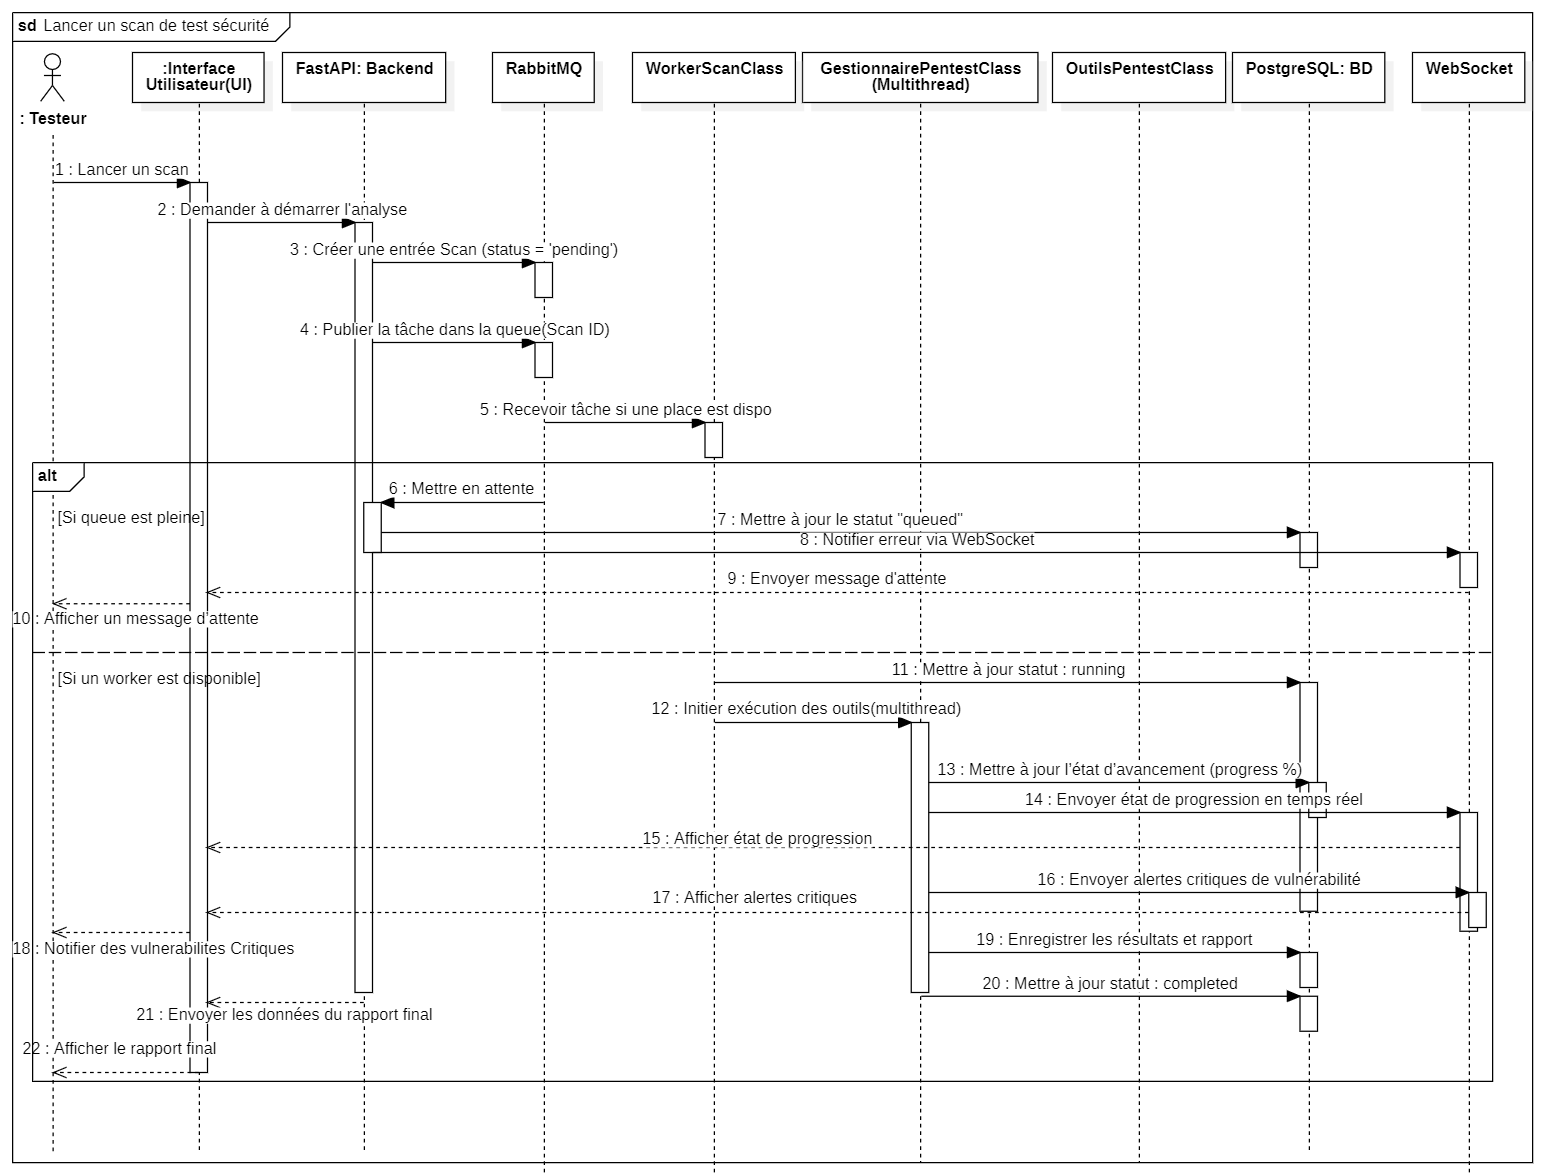
\includegraphics[width=\linewidth]{chapitres/ch3Sp1/section/sprint2/img/seq-lancerSp1.2.png}
    \caption{\centering Diagramme de séquence de conception de cas «Lancer un scan de test sécurité»}
    \label{fig:seq1ScanAnalyse}
\end{figure}
\vspace{-0.6cm}

%     \section{Réalisation du sprint 1.2}
%     Dans cette section, nous présentons les principales interfaces réalisées au cours du sprint 1.2. 
\begin{itemize}[label=$\bullet$]
    \item \textbf{Interface de configuration des paramètres de scan}:
    La figure \ref{fig:interface_parametres_scan}\footnote{Voir Annexe E, figure \ref{fig:interface_parametres_scan}} illustre l’interface permettant de personnaliser les paramètres d’un scan. Celle-ci permet à l’utilisateur de définir la profondeur de l’analyse, d’activer ou non certains modules (comme le spider ou le scan AJAX), ou encore de choisir des options spécifiques à certains outils.
    
    \item \textbf{Interface de sélection des outils de sécurité}:
    La figure \ref{fig:interface_selection_outils} présente l’écran dédié à la sélection des outils de sécurité. Cette interface propose une liste de cases à cocher pour activer ou désactiver les outils disponibles, accompagnée de boutons «Tout sélectionner» et «Tout désélectionner». Les préférences de l’utilisateur sont sauvegardées pour les réutiliser dans les futurs scans.
     \begin{figure}[H]
        \centering
        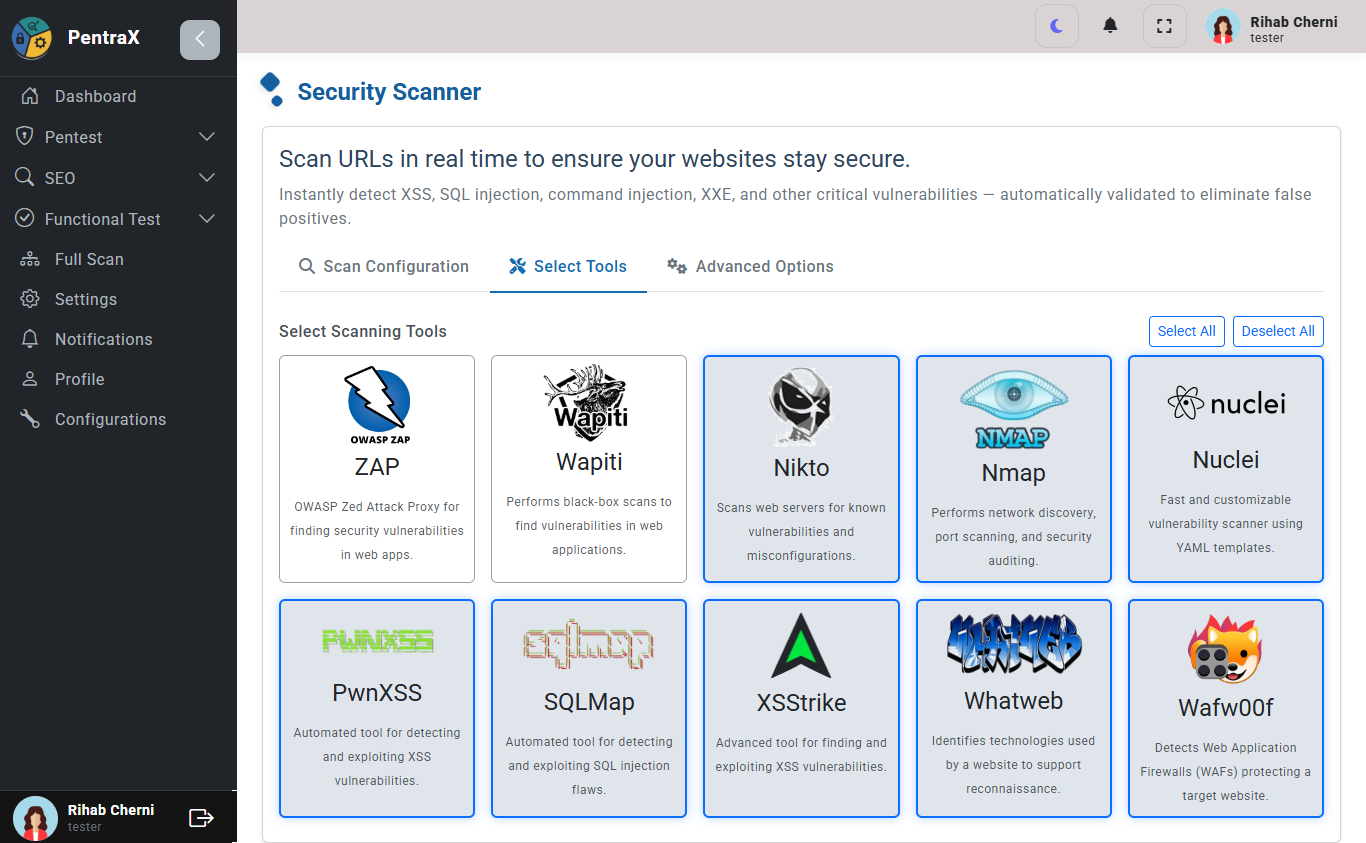
\includegraphics[width=\textwidth]{chapitres/ch3Sp1/section/sprint2/img/interface/tools.png}
        \caption{Interface de sélection des outils de sécurité}
        \label{fig:interface_selection_outils}
    \end{figure}
    \vspace{-0.2cm}
    \item \textbf{Interface utilisateur pour le lancement de scans, avec ou sans authentification} :\\
        La figure \ref{fig:interface_lancement_scan} illustre le formulaire principal de lancement d’un test de sécurité. L’utilisateur y renseigne l’URL de la cible, choisit les outils à utiliser, configure les paramètres du scan, puis lance l’analyse via un bouton dédié.

        Cette interface propose également une section dédiée à l’authentification, activable via des boutons radio. En fonction du type sélectionné, les champs correspondants s’affichent dynamiquement : identifiants (nom d’utilisateur et mot de passe), jetons d’accès (tokens), ou cookies de session. Cette fonctionnalité est essentielle pour analyser les zones protégées d’une application web. Pour plus de détails sur le lancement des scans de sécurité, la gestion des paramètres d’authentification et la configuration des outils, voir l’annexe C\footnote{Voir Annexe C: Automatisation des outils de pentesting}.
        \begin{figure}[H]
            \centering
            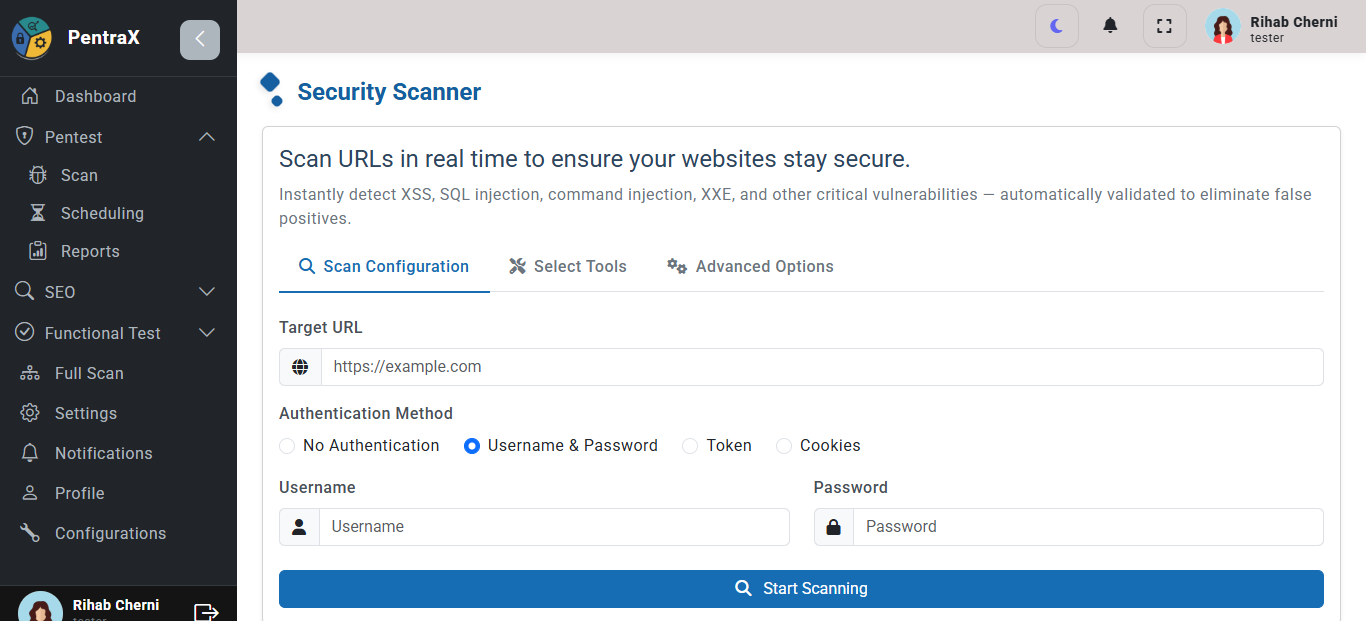
\includegraphics[width=\textwidth]{chapitres/ch3Sp1/section/sprint2/img/interface/start-sca.PNG}
            \caption{Interface de lancement de scan avec ou sans authentification}
            \label{fig:interface_lancement_scan}
        \end{figure}
        \vspace{-0.2cm}
    \item \textbf{Interface de suivi en temps réel des scans}: Comme illustré dans la figure \ref{fig:interface_suivi_ws}\footnote{Voir Annexe E, figure \ref{fig:interface_suivi_ws}}, cette interface permet de suivre l’évolution du scan en temps réel grâce à l’intégration des WebSockets, avec un indicateur de progression affiché de 0 à 100\,\%.    
    \item \textbf{Interface de visualisation des résultats}:
    La figure \ref{fig:interface_resultats_scan} montre l’écran de consultation des vulnérabilités détectées. Des filtres par type, gravité ou outil sont proposés pour affiner l’analyse, et chaque vulnérabilité est accompagnée d’un résumé, de son risque, de sa source et d’une suggestion de correction.
        \begin{figure}[H]
            \centering
            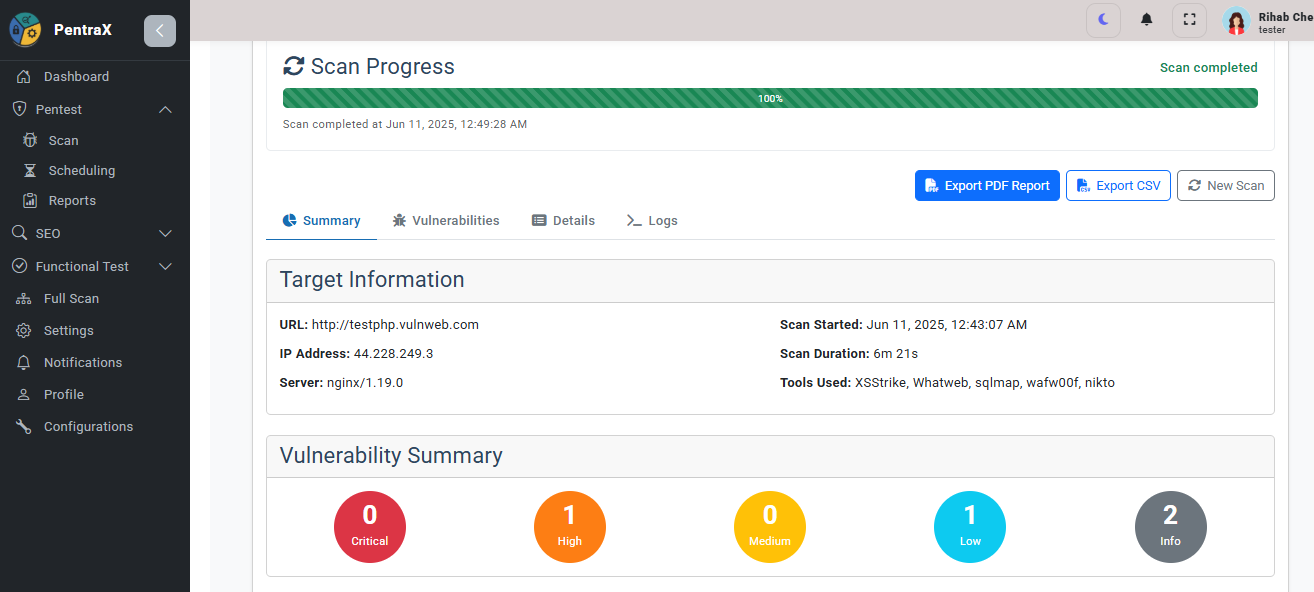
\includegraphics[width=\textwidth]{chapitres/ch3Sp1/section/sprint2/img/interface/res1.PNG}
            \caption{\centering Interface de visualisation des résultats de scan (premier onglet : statistiques et détails techniques)}
            \label{fig:interface_resultats_scan}
        \end{figure}
        \vspace{-0.2cm}
    \item \textbf{Interface de l’historique des scans}:
    L’interface illustrée par la figure \ref{fig:interface_historique_scans}\footnote{Voir Annexe E, figure \ref{fig:interface_historique_scans}} permet d’accéder aux rapports précédemment générés. Une table paginée présente les scans enregistrés, accompagnée de filtres, d’un champ de recherche, et d’une option de suppression.
    
    \item \textbf{Interface de téléchargement des rapports}:
    Comme présenté dans la figure \ref{fig:interface_export_rapports}\footnote{Voir Annexe E, figure \ref{fig:interface_export_rapports}}, cette interface permet de télécharger les rapports aux formats JSON, PDF ou CSV, selon les besoins de l’utilisateur.


    \item \textbf{Interface pour le paramétrage des canaux de diffusion} : La figure \ref{fig:interface_parametrage_canaux}\footnote{Voir Annexe E, figure \ref{fig:interface_parametrage_canaux}} illustre l’interface dédiée à la configuration détaillée des canaux de diffusion des rapports. Elle permet à l’utilisateur de spécifier, pour chaque type de test (sécurité, SEO, fonctionnel), les canaux de notification souhaités (Slack, Jira, Email), le format du rapport associé (PDF, HTML, JSON). Des champs dynamiques permettent d’ajouter plusieurs destinataires e-mail et d’entrer des clés API sécurisées pour Slack et Jira. Cette interface vise à centraliser et automatiser la diffusion ciblée des rapports vers les bons interlocuteurs.

    \item \textbf{Interface d’intégration Jira}:
    La figure \ref{fig:interface_jira_integration}\footnote{Voir Annexe E, figure \ref{fig:interface_jira_integration}} illustre la fonctionnalité d’envoi des vulnérabilités détectées directement vers Jira pour créer automatiquement des tickets. Un aperçu des tickets créés est également affiché.
    
    \item \textbf{Interface de notification Slack et e-mail}:
    Les figures \ref{fig:interface_slack_notification} et \ref{fig:interface_email_notification}\footnote{Voir Annexe E, figures \ref{fig:interface_slack_notification} et \ref{fig:interface_email_notification}} présentent respectivement l’envoi automatique des rapports via Slack et e-mail. Ces notifications sont déclenchées à la fin du scan, contenant un résumé des vulnérabilités et un lien vers le rapport complet.
    
    \item \textbf{Interface de planification automatique des scans}:  
    La figure \ref{fig:interface_planification_scan}\footnote{Voir Annexe E, figure \ref{fig:interface_planification_scan}} illustre l’écran de planification permettant à l’utilisateur de définir des scans récurrents. Il peut spécifier la fréquence (quotidienne, hebdomadaire, mensuelle), l’heure d’exécution, la cible concernée et les paramètres associés. Une liste des tâches planifiées est également visible et modifiable.
    
    \item \textbf{Interface de gestion centralisée des notifications}: La figure \ref{fig:interface_notifications_config}\footnote{Voir Annexe E, figure \ref{fig:interface_notifications_config}} présente une interface unifiée permettant à l’utilisateur d’activer et de configurer les canaux de diffusion des rapports vers Jira, Slack et l’e-mail. L’interface offre des options pour sélectionner les canaux souhaités, saisir les identifiants API (Slack, Jira ou les adresses e-mail), et choisir les formats (HTML, PDF, JSON) ainsi que les types de rapports à transmettre (sécurité, fonctionnel, SEO).
\end{itemize}


    \section*{\texorpdfstring{Conclusion}{Conclusion}}
    \addcontentsline{toc}{chapter}{\textbf{Conclusion}}
    \begin{justify}
Ce premier sprint a constitué une étape fondamentale dans le développement de notre application, avec l’implémentation de l’authentification, de la gestion des utilisateurs, des scans de sécurité et des notifications en temps réel. Le sprint suivant visera à enrichir ces fonctionnalités, à améliorer l’ergonomie et à poursuivre l’automatisation des tests fonctionnels et SEO.
\end{justify}

\end{justify}   